\documentclass{notes}
\usetikzlibrary{shapes, shapes.geometric}
\usepackage{multirow,bigdelim}

\class{CS 181 (Introduction to Formal Languages and Automata Theory)}

\begin{document}

\section{Deterministic finite automata (DFAs)}

\subsection{Basic notions}

\begin{defn}
  An \textbf{alphabet} is any finite set of symbols.
\end{defn}

\begin{eg}
  Binary alphabet: $\left \{ \verb~0~, \verb~1~ \right \}$
\end{eg}

\begin{eg}
  English alphabet: $\left \{ \verb~a~, \verb~b~, \dots, \verb~c~ \right \}$
\end{eg}

\begin{defn}
  A \textbf{string} is any finite sequence of symbols from a given alphabet.
\end{defn}

\begin{eg}
  \verb~001010110101~
\end{eg}

\begin{eg}
  \verb~abracadabra~
\end{eg}

\begin{eg}
  $\varepsilon$ (empty string)
\end{eg}

\begin{defn}
  A \textbf{language} is a set of strings over a given alphabet.
\end{defn}

\begin{eg}
  $\varnothing$ (empty language)
\end{eg}

\begin{eg}
  $\left \{ \varepsilon \right \}$
\end{eg}

\begin{eg}
  $\left \{ \verb~acclaim~, \verb~aim~, \verb~brim~, \dots \right \}$
\end{eg}

\begin{eg}
  $\left \{ \verb~0~, \verb~1~, \verb~00~, \verb~11~, \dots \right \}$
\end{eg}

\begin{defn}
  A \textbf{computational device} is a mechanism that inputs a string and either accepts or rejects it.
\end{defn}

\subsection{Deterministic finite automata}

\begin{itemize}
  \item Choose an alphabet: $\left \{ \verb~a~, \verb~b~ \right \}$.
  \item Draw states.
  \item Choose start state and accept states.
  \item Draw transitions (out of every state on every symbol).
\end{itemize}

\begin{minipage}{0.5 \textwidth}
  \begin{center}
    \begin{tikzpicture}[> = stealth, node distance = 3em]
      \node[initial, initial text=, state, minimum size = 2em] (q1) {};
      \node[below left = of q1, accepting, state, minimum size = 2em] (q2) {};
      \node[below right = of q1, accepting, state, minimum size = 2em] (q3) {};
      \node[below right = of q2, state, minimum size = 2em] (q4) {};
      \draw[->]
      (q1) edge[above left] node{\verb~a~} (q2)
      (q1) edge[above right] node{\verb~b~} (q3)
      (q2) edge[loop left] node{\verb~a~} (q2)
      (q2) edge[below left] node{\verb~b~} (q4)
      (q3) edge[below right] node{\verb~a~} (q4)
      (q3) edge[loop right] node{\verb~b~} (q3)
      (q4) edge[loop below] node{\verb~a~,\verb~b~} (q4)
      ;
    \end{tikzpicture}
  \end{center}
\end{minipage}%
\begin{minipage}{0.5 \textwidth}
  \begin{center}
    \begin{tabular}{cc}
      Input & Output \\ 
      \hline
      $\varepsilon$ & reject \\ 
      \verb~ab~ & reject \\ 
      \verb~aaa~ & accept \\ 
      \verb~bb~ & accept
    \end{tabular}
  \end{center}
\end{minipage}

In words, this machine accepts nonempty strings of all \verb~a~'s or all \verb~b~'s.

\begin{defn}
  The \textbf{language} of a DFA is the set of all strings it accepts.
\end{defn}

\begin{eg}
  
  \begin{minipage}{0.5 \textwidth}
    \begin{center}
      \begin{tikzpicture}[> = stealth, node distance = 3em]
        \node[accepting, initial, initial text=, state, minimum size = 2em] (q1) at (90 : 1.5) {};
        \node[state, minimum size = 2em] (q2) at (330 : 1.5) {};
        \node[state, minimum size = 2em] (q3) at (210 : 1.5) {};
        \draw[->]
        (q1) edge[loop above] node{\verb~0~} (q1)
        (q1) edge[below left] node{\verb~1~} (q2)
        (q1) edge[bend right, above left] node{\verb~2~} (q3)
        (q2) edge[loop right] node{\verb~0~} (q2)
        (q2) edge[above] node{\verb~1~} (q3)
        (q2) edge[bend right, above right] node{\verb~2~} (q1)
        (q3) edge[loop left] node{\verb~0~} (q3)
        (q3) edge[below right] node{\verb~1~} (q1)
        (q3) edge[bend right, below] node{\verb~2~} (q2)
        ;
      \end{tikzpicture}
    \end{center}
  \end{minipage}%
  \begin{minipage}{0.5 \textwidth}
    \begin{center}
      \begin{tabular}{cc}
        Input & Output \\ 
        \hline
        \verb~00...0~ & accept \\ 
        \verb~12~ & accept \\ 
        \verb~111~ & accept \\ 
        \verb~20~ & reject \\ 
        \verb~1~ & reject
      \end{tabular}
    \end{center}
  \end{minipage}

  \begin{center}
    $\Sigma = \left \{ \verb~0~, \verb~1~, \verb~2~ \right \}$, $\mathcal L = \left \{ w : 3 \mid \sum w_i \right \}$
  \end{center}
\end{eg}

\begin{eg}
  \begin{center}
    \begin{tikzpicture}[> = stealth, node distance = 3em]
      \node[accepting, initial, initial text=, state, minimum size = 2em] (q1) {};
      \node[right = of q1, state, minimum size = 2em] (q2) {};
      \draw[->]
      (q1) edge[bend right, below] node{\verb~0~,\verb~1~} (q2)
      (q2) edge[bend right, above] node{\verb~0~,\verb~1~} (q1)
      ;
    \end{tikzpicture}

    $\Sigma = \left \{ \verb~0~, \verb~1~ \right \}$, $\mathcal L = \left \{ w : 2 \mid \left | w \right | \right \}$
  \end{center}
\end{eg}

\begin{eg}
  \begin{center}
    \begin{tikzpicture}[> = stealth, node distance = 3em]
      \node[initial, initial text=, state, minimum size = 2em] (q1) {};
      \node[accepting, below left = of q1, state, minimum size = 2em] (q2) {};
      \node[below = of q2, state, minimum size = 2em] (q3) {};
      \node[accepting, below right = of q1, state, minimum size = 2em] (q4) {};
      \node[below = of q4, state, minimum size = 2em] (q5) {};
      \draw[->]
      (q1) edge[above left] node{\verb~a~} (q2)
      (q1) edge[above right] node{\verb~b~} (q4)
      (q2) edge[loop left] node{\verb~a~} (q2)
      (q2) edge[bend right, left] node{\verb~b~} (q3)
      (q3) edge[bend right, right] node{\verb~a~} (q2)
      (q3) edge[loop below] node{\verb~b~} (q3)
      (q4) edge[bend right, left] node{\verb~a~} (q5)
      (q4) edge[loop right] node{\verb~b~} (q4)
      (q5) edge[loop below] node{\verb~a~} (q5)
      (q5) edge[bend right, right] node{\verb~b~} (q4)
      ;
    \end{tikzpicture}

    $\Sigma = \left \{ \verb~a~, \verb~b~ \right \}$, $\mathcal L = \left \{ w : w \neq \varepsilon \land w_1 = w_{\left | w \right |  } \right \}$
  \end{center}
\end{eg}

\subsection{Designing DFAs}

We will be using the binary alphabet $\left \{ \verb~0~, \verb~1~ \right \}$.

\begin{eg}
  A DFA for $\mathcal L = \varnothing$ is given by: 
  
  \begin{center}
    \begin{tikzpicture}[> = stealth, node distance = 3em]
      \node[initial, initial text=, state, minimum size = 2em] (q1) {};
      \draw[->]
      (q1) edge[loop right] node{\verb~0~,\verb~1~} (q1)
      ;
    \end{tikzpicture}
  \end{center}
\end{eg}

\begin{eg}
  A DFA for $\mathcal L = \left \{ w : \text{every odd position is a \verb~1~} \right \}$ is given by: 
  
  \begin{center}
    \begin{tikzpicture}[> = stealth, node distance = 3em]
      \node[accepting, initial, initial text=, state, minimum size = 2em] (q1) {};
      \node[accepting, below right = of q1, state, minimum size = 2em] (q2) {};
      \node[above right = of q1, state, minimum size = 2em] (q3) {};
      \draw[->]
      (q1) edge[above left] node{\verb~0~} (q3)
      (q1) edge[bend right, below left] node{\verb~1~} (q2)
      (q2) edge[bend right, above right] node{\verb~0~,\verb~1~} (q1)
      (q3) edge[loop right] node{\verb~0~,\verb~1~} (q3)
      ;
    \end{tikzpicture}
  \end{center}
\end{eg}

\begin{eg}
  A DFA for $\mathcal L = \left \{ w : \text{$w$ ends in \verb~0~} \right \}$ is given by: 
  
  \begin{center}
    \begin{tikzpicture}[> = stealth, node distance = 3em]
      \node[initial, initial text=, state, minimum size = 2em] (q1) {};
      \node[right = of q1, accepting, state, minimum size = 2em] (q2) {};
      \draw[->]
      (q1) edge[bend right, below] node{\verb~0~} (q2)
      (q1) edge[loop above] node{\verb~1~} (q1)
      (q2) edge[loop below] node{\verb~0~} (q2)
      (q2) edge[bend right, above] node{\verb~1~} (q1)
      ;
    \end{tikzpicture}
  \end{center}
\end{eg}

\begin{eg}
  A DFA for $\mathcal L = \left \{ w : \text{$w$ begins with \verb~1~, ends with \verb~0~} \right \}$ is given by: 
  
  \begin{center}
    \begin{tikzpicture}[> = stealth, node distance = 3em]
      \node[initial, initial text=, state, minimum size = 2em] (q1) {};
      \node[above right = of q1, state, minimum size = 2em] (q2) {};
      \node[right = of q2, accepting, state, minimum size = 2em] (q3) {};
      \node[below right = of q1, state, minimum size = 2em] (q4) {};
      \draw[->]
      (q1) edge[below left] node{\verb~0~} (q4)
      (q1) edge[above left] node{\verb~1~} (q2)
      (q2) edge[bend right, below] node{\verb~0~} (q3)
      (q2) edge[loop above] node{\verb~1~} (q2)
      (q3) edge[loop right] node{\verb~0~} (q3)
      (q3) edge[bend right, above] node{\verb~1~} (q2)
      (q4) edge[loop right] node{\verb~0~,\verb~1~} (q4)
      ;
    \end{tikzpicture}
  \end{center}
\end{eg}

\begin{eg}
  A DFA for $\mathcal L = \left \{ w : \left | w \right | \leq 4  \right \}$ is given by: 
  
  \begin{center}
    \begin{tikzpicture}[> = stealth, node distance = 3em]
      \node[accepting, initial, initial text=, state, minimum size = 2em] (q1) {};
      \node[right = of q1, accepting, state, minimum size = 2em] (q2) {};
      \node[accepting, right = of q2, state, minimum size = 2em] (q3) {};
      \node[accepting, right = of q3, state, minimum size = 2em] (q4) {};
      \node[accepting, right = of q4, state, minimum size = 2em] (q5) {};
      \node[right = of q5, state, minimum size = 2em] (q6) {};
      \draw[->]
      (q1) edge[above] node{\verb~0~,\verb~1~} (q2)
      (q2) edge[above] node{\verb~0~,\verb~1~} (q3)
      (q3) edge[above] node{\verb~0~,\verb~1~} (q4)
      (q4) edge[above] node{\verb~0~,\verb~1~} (q5)
      (q5) edge[above] node{\verb~0~,\verb~1~} (q6)
      (q6) edge[loop right] node{\verb~0~,\verb~1~} (q6)
      ;
    \end{tikzpicture}
  \end{center}
\end{eg}

\newpage

\begin{eg}
  A DFA for $\mathcal L = \left \{ w : 1000 \mid \left | w \right | \right \}$ is given by: 
  
  In words, each state represents a remainder modulo 1000, and only the 0 state is accepting.
\end{eg}

\begin{eg}
  A DFA for $\mathcal L = \left \{ w : \text{$w$ contains \verb~0101~ as a substring} \right \}$ is given by: 
  
  \begin{center}
    \begin{tikzpicture}[> = stealth, node distance = 3em]
      \node[initial, initial text=, state, minimum size = 2em] (q1) {$\varepsilon$};
      \node[right = of q1, state, minimum size = 2em] (q2) {\verb~0~};
      \node[right = of q2, state, minimum size = 2em] (q3) {\verb~01~};
      \node[right = of q3, state, minimum size = 2em] (q4) {\verb~010~};
      \node[accepting, right = of q4, state, minimum size = 2em] (q5) {\verb~0101~};
      \draw[->]
      (q1) edge[above] node{\verb~0~} (q2)
      (q1) edge[loop above] node{\verb~1~} (q1)
      (q2) edge[loop above] node{\verb~0~} (q2)
      (q2) edge[above] node{\verb~1~} (q3)
      (q3) edge[above] node{\verb~0~} (q4)
      (q3) edge[bend right = 75, above] node{\verb~1~} (q1)
      (q4) edge[bend right = 60, above] node{\verb~0~} (q2)
      (q4) edge[above] node{\verb~1~} (q5)
      (q5) edge[loop right] node{\verb~0~,\verb~1~} (q5)
      ;
    \end{tikzpicture}
  \end{center}
\end{eg}

\begin{eg}[Week 1 Discussion]
  A DFA for $\mathcal L = \left \{ w : \left | w \right | > 0 \land \text{$w$ contains only \verb~1~s} \right \}$ is given by: 
  
  \begin{center}
    \begin{tikzpicture}[> = stealth, node distance = 3em]
      \node[initial, initial text=, state, minimum size = 2em] (q1) {};
      \node[right = of q1, accepting, state, minimum size = 2em] (q2) {};
      \node[right = of q2, state, minimum size = 2em] (q3) {};
      \draw[->]
      (q1) edge[bend right, below] node{\verb~0~} (q3)
      (q1) edge[above] node{\verb~1~} (q2)
      (q2) edge[above] node{\verb~0~} (q3)
      (q2) edge[loop above] node{\verb~1~} (q2)
      (q3) edge[loop right] node{\verb~0~,\verb~1~} (q3)
      ;
    \end{tikzpicture}
  \end{center}
\end{eg}

\begin{eg}[Week 1 Discussion]
  A DFA for $\mathcal L = \left \{ w : \text{$w$ ends in \verb~1101~} \right \}$ is given by: 
  
  \begin{center}
    \begin{tikzpicture}[> = stealth, node distance = 3em]
      \node[initial, initial text=, state, minimum size = 2em] (q1) {};
      \node[right = of q1, state, minimum size = 2em] (q2) {};
      \node[right = of q2, state, minimum size = 2em] (q3) {};
      \node[right = of q3, state, minimum size = 2em] (q4) {};
      \node[accepting, right = of q4, state, minimum size = 2em] (q5) {};
      \draw[->]
      (q1) edge[loop below] node{\verb~0~} (q1)
      (q1) edge[bend right, below] node{\verb~1~} (q2)
      (q2) edge[bend right, above] node{\verb~0~} (q1)
      (q2) edge[above] node{\verb~1~} (q3)
      (q3) edge[above] node{\verb~0~} (q4)
      (q3) edge[loop above] node{\verb~1~} (q3)
      (q4) edge[bend right = 60, above] node{\verb~0~} (q1)
      (q4) edge[above] node{\verb~1~} (q5)
      (q5) edge[bend right = 75, above] node{\verb~0~} (q1)
      (q5) edge[bend right, above] node{\verb~1~} (q3)
      ;
    \end{tikzpicture}
  \end{center}
\end{eg}

\begin{eg}[Week 1 Discussion]
  A DFA for $\mathcal L = \left \{ w : \text{$w$ contains \verb~1101~} \right \}$ is given by: 
  
  \begin{center}
    \begin{tikzpicture}[> = stealth, node distance = 3em]
      \node[initial, initial text=, state, minimum size = 2em] (q1) {};
      \node[right = of q1, state, minimum size = 2em] (q2) {};
      \node[right = of q2, state, minimum size = 2em] (q3) {};
      \node[right = of q3, state, minimum size = 2em] (q4) {};
      \node[accepting, right = of q4, state, minimum size = 2em] (q5) {};
      \draw[->]
      (q1) edge[loop below] node{\verb~0~} (q1)
      (q1) edge[bend right, below] node{\verb~1~} (q2)
      (q2) edge[bend right, above] node{\verb~0~} (q1)
      (q2) edge[above] node{\verb~1~} (q3)
      (q3) edge[above] node{\verb~0~} (q4)
      (q3) edge[loop above] node{\verb~1~} (q3)
      (q4) edge[bend right = 60, above] node{\verb~0~} (q1)
      (q4) edge[above] node{\verb~1~} (q5)
      (q5) edge[loop right] node{\verb~0~,\verb~1~} (q5)
      ;
    \end{tikzpicture}
  \end{center}
\end{eg}

\newpage

\subsection{Formal definitions}

\begin{defn}
  A DFA is a tuple $(Q, \Sigma, \delta, q_{0}, F)$
  where
  \begin{itemize}
    \item $Q =$ set of states, 
    \item $\Sigma =$ alphabet, 
    \item $\delta =$ transition function ($\delta \colon Q \times \Sigma \to Q$), 
    \item $q_0 =$ start state ($q_0 \in Q$), and 
    \item $F =$ set of accept states ("favorable"? states, $F \subseteq Q$).
  \end{itemize}
\end{defn}

\begin{eg}
  A formal description of the DFA

  \begin{center}
    \begin{tikzpicture}[> = stealth, node distance = 3em]
      \node[initial, initial text=, state, minimum size = 2em] (q1) {$A$};
      \node[accepting, right = of q1, accepting, state, minimum size = 2em] (q2) {$B$};
      \node[right = of q2, state, minimum size = 2em] (q3) {$C$};
      \draw[->]
      (q1) edge[loop above] node{\verb~0~} (q1)
      (q1) edge[above] node{\verb~1~} (q2)
      (q2) edge[bend right, below] node{\verb~0~} (q3)
      (q2) edge[loop above] node{\verb~1~} (q2)
      (q3) edge[bend right, above] node{\verb~0~,\verb~1~} (q2)
      ;
    \end{tikzpicture}
  \end{center}
  
  is given by $(\left \{ A, B, C \right \}, \left \{ \verb~0~, \verb~1~ \right \}, \delta, A, \left \{ B \right \})$ where $\delta$ is defined by the table
  \begin{center}
    \begin{tabular}{c|cc}
      & \verb~0~ & \verb~1~ \\ 
      \hline
      $A$ & $A$ & $B$ \\ 
      $B$ & $C$ & $B$ \\ 
      $C$ & $B$ & $B$.
    \end{tabular}
  \end{center}
\end{eg}

\begin{eg}
  The graph for the DFA $(\left \{ A, B, C, D, E \right \}, \left \{ \verb~0~, \verb~1~ \right \}, \delta, C, \left \{ C \right \})$ where $\delta$ is defined by the table 
  \begin{center}
    \begin{tabular}{c|cc}
      & \verb~0~ & \verb~1~ \\ 
      \hline
      $A$ & $A$ & $B$ \\ 
      $B$ & $A$ & $C$ \\ 
      $C$ & $B$ & $D$ \\ 
      $D$ & $C$ & $E$ \\ 
      $E$ & $D$ & $E$
    \end{tabular}
  \end{center}
  
  is given by: 
  
  \begin{center}
    \begin{tikzpicture}[> = stealth, node distance = 3em]
      \node[state, minimum size = 2em] (q1) {$A$};
      \node[right = of q1, state, minimum size = 2em] (q2) {$B$};
      \node[accepting, initial above, initial text=, right = of q2, state, minimum size = 2em] (q3) {$C$};
      \node[right = of q3, state, minimum size = 2em] (q4) {$D$};
      \node[right = of q4, state, minimum size = 2em] (q5) {$E$};
      \draw[->]
      (q1) edge[loop left] node{\verb~0~} (q1)
      (q1) edge[bend right, below] node{\verb~1~} (q2)
      (q2) edge[bend right, above] node{\verb~0~} (q1)
      (q2) edge[bend right, below] node{\verb~1~} (q3)
      (q3) edge[bend right, above] node{\verb~0~} (q2)
      (q3) edge[bend right, below] node{\verb~1~} (q4)
      (q4) edge[bend right, above] node{\verb~0~} (q3)
      (q4) edge[bend right, below] node{\verb~1~} (q5)
      (q5) edge[bend right, above] node{\verb~0~} (q4)
      (q5) edge[loop right] node{\verb~1~} (q5)
      ;
    \end{tikzpicture}
  \end{center}
\end{eg}

\begin{eg}
  A formal description for Example~\ref{eg:1.3.6} is given by $(\left \{ 0, 1, 2, \dots, 999 \right \}, \left \{ \verb~0~, \verb~1~ \right \}, \delta, 0, \left \{ 0 \right \})$ where $\delta(q, \sigma) = (q + 1) \mod 1000$.
\end{eg}

\newpage

\begin{defn}
  DFA $(Q, \Sigma, \delta, q_{0}, F)$ {\boldmath \bfseries accepts} a string $w = w_1 w_2 \dots w_n$ iff
  \[
    \delta(\cdots \delta(\delta(q_0, w_1), w_2) \cdots, w_n) \in F.
  \]
\end{defn}

\begin{defn}
  DFA $D$ {\boldmath \bfseries recognizes} the language $\mathcal L$ iff 
  \[
    \mathcal L = \left \{ w : \text{$D$ accepts $w$} \right \}.
  \]
\end{defn}

\begin{note}
  \begin{itemize}
    \item Every DFA recognizes exactly 1 language.

    \item A language has either 0 or $\infty$ DFAs recognizing it.
  \end{itemize}
\end{note}

\section{Nondeterminism}

\subsection{Basic notions}

\begin{eg}
  \begin{center}
    \begin{tikzpicture}[> = stealth, node distance = 3em]
      \node[initial, initial text=, state, minimum size = 2em] (q1) {$A$};
      \node[right = of q1, state, minimum size = 2em] (q2) {$B$};
      \node[right = of q2, state, minimum size = 2em] (q3) {$C$};
      \node[accepting, right = of q3, state, minimum size = 2em] (q4) {$D$};
      \draw[->]
      (q1) edge[loop above] node{\verb~0~,\verb~1~} (q1)
      (q1) edge[above] node{\verb~1~} (q2)
      (q2) edge[above] node{\verb~0~,$\varepsilon$} (q3)
      (q3) edge[above] node{\verb~1~} (q4)
      (q4) edge[loop above] node{\verb~0~,\verb~1~} (q4)
      ;
    \end{tikzpicture}
  \end{center}

  \begin{itemize}
    \item Choose an alphabet: $\left \{ \verb~0~, \verb~1~ \right \}$.

    \item Draw states.
      
    \item Choose start state and accept states.
    The steps so far are the same as those of a DFA.
      
    \item Draw transitions.
    A state may have any number of transitions on a given symbol.
    A state may also have transitions on $\varepsilon$.
  \end{itemize}
\end{eg}

\begin{defn}
  An NFA {\boldmath \bfseries accepts} $w$ iff there is \textit{at least} one path to an accept state.
\end{defn}

\newpage

\begin{eg}
  The output table for Example~\ref{eg:2.1.1} is given by 
  \begin{center}
    \begin{tabular}{ccc}
      Input & Accepting path & Output \\ 
      \hline
      $\varepsilon$ & - & reject \\ 
      \verb~0~ & - & reject \\ 
      \verb~1~ & - & reject \\ 
      \verb~010110~ & $AABCDDD$ & accept \\
      \verb~010~ & - & reject \\ 
      \verb~11~ & $ABCD$ & accept. 
    \end{tabular}
  \end{center}
  
  Then the language is the set of all strings containing \verb~101~ or \verb~11~.
\end{eg}

\subsection{Using shortcuts}

\begin{eg}
  An NFA for $\mathcal L = \varnothing$ is given by: 
  
  \begin{center}
    \begin{tikzpicture}[> = stealth, node distance = 3em]
      \node[initial, initial text=, state, minimum size = 2em] (q1) {};
      \draw[->]
      ;
    \end{tikzpicture}
  \end{center}
\end{eg}

\begin{eg}
  An NFA for $\mathcal L = \left \{ \varepsilon \right \}$ is given by: 

  \begin{center}
    \begin{tikzpicture}[> = stealth, node distance = 3em]
      \node[accepting, initial, initial text=, state, minimum size = 2em] (q1) {};
      \draw[->]
      ;
    \end{tikzpicture}
  \end{center}
\end{eg}

\begin{eg}
  An NFA for $\mathcal L = \left \{ w : \text{$w$ doesn't contain \verb~1~} \right \}$ is given by: 

  \begin{center}
    \begin{tikzpicture}[> = stealth, node distance = 3em]
      \node[accepting, initial, initial text=, state, minimum size = 2em] (q1) {};
      \draw[->]
      (q1) edge[loop right] node{\verb~0~} (q1)
      ;
    \end{tikzpicture}
  \end{center}
\end{eg}

\begin{eg}
  An NFA for $\mathcal L = \left \{ w : \text{$\left | w \right | \geq 2$ and $w$ starts and ends with \verb~0~} \right \}$ is given by: 
  
  \begin{center}
    \begin{tikzpicture}[> = stealth, node distance = 3em]
      \node[initial, initial text=, state, minimum size = 2em] (q1) {};
      \node[right = of q1, state, minimum size = 2em] (q2) {};
      \node[accepting, right = of q2, state, minimum size = 2em] (q3) {};
      \draw[->]
      (q1) edge[above] node{\verb~0~} (q2)
      (q2) edge[above] node{\verb~0~} (q3)
      (q2) edge[loop above] node{\verb~0~,\verb~1~} (q2)
      ;
    \end{tikzpicture}
  \end{center}
\end{eg}

\subsection{Pattern matching}

\begin{eg}
  An NFA for $\mathcal L = \left \{ w : \text{conatins \verb~0101~} \right \}$ is given by: 
  
  \begin{center}
    \begin{tikzpicture}[> = stealth, node distance = 3em]
      \node[initial, initial text=, state, minimum size = 2em] (q1) {};
      \node[right = of q1, state, minimum size = 2em] (q2) {};
      \node[right = of q2, state, minimum size = 2em] (q3) {};
      \node[right = of q3, state, minimum size = 2em] (q4) {};
      \node[accepting, right = of q4, state, minimum size = 2em] (q5) {};
      \draw[->]
      (q1) edge[loop above] node{\verb~0~,\verb~1~} (q1)
      (q1) edge[above] node{\verb~0~} (q2)
      (q2) edge[above] node{\verb~1~} (q3)
      (q3) edge[above] node{\verb~0~} (q4)
      (q4) edge[above] node{\verb~1~} (q5)
      (q5) edge[loop above] node{\verb~0~,\verb~1~} (q5)
      ;
    \end{tikzpicture}
  \end{center}
\end{eg}

\newpage

\begin{eg}
  An NFA for $\mathcal L = \{ w : w = \underbrace{\verb~00...0~}_{\geq 0}\underbrace{\verb~11...1~}_{\geq 0}\underbrace{\verb~00...0~}_{\geq 1} \}$ is given by: 
  
  \begin{center}
    \begin{tikzpicture}[> = stealth, node distance = 3em]
      \node[initial, initial text=, state, minimum size = 2em] (q1) {};
      \node[right = of q1, state, minimum size = 2em] (q2) {};
      \node[accepting, right = of q2, state, minimum size = 2em] (q3) {};
      \draw[->]
      (q1) edge[loop above] node{\verb~0~} (q1)
      (q1) edge[above] node{$\varepsilon$} (q2)
      (q2) edge[loop above] node{\verb~1~} (q2)
      (q2) edge[above] node{\verb~0~} (q3)
      (q3) edge[loop above] node{\verb~0~} (q3)
      ;
    \end{tikzpicture}
  \end{center}
\end{eg}

\begin{eg}
  An NFA for $\mathcal L = \left \{ w : \text{$w$ has a \verb~1~ in the 3rd position from the end} \right \}$ is given by: 
  
  \begin{center}
    \begin{tikzpicture}[> = stealth, node distance = 3em]
      \node[initial, initial text=, state, minimum size = 2em] (q1) {};
      \node[right = of q1, state, minimum size = 2em] (q2) {};
      \node[right = of q2, state, minimum size = 2em] (q3) {};
      \node[accepting, right = of q3, state, minimum size = 2em] (q4) {};
      \draw[->]
      (q1) edge[loop above] node{\verb~0~,\verb~1~} (q1)
      (q1) edge[above] node{\verb~1~} (q2)
      (q2) edge[above] node{\verb~0~,\verb~1~} (q3)
      (q3) edge[above] node{\verb~0~,\verb~1~} (q4)
      ;
    \end{tikzpicture}
  \end{center}
\end{eg}

\begin{eg}[Week 1 Discussion]
  An NFA for $\mathcal L = \left \{ w : \text{$w$ contains \verb~1101~} \right \}$ is given by: 
  
  \begin{center}
    \begin{tikzpicture}[> = stealth, node distance = 3em]
      \node[initial, initial text=, state, minimum size = 2em] (q1) {};
      \node[right = of q1, state, minimum size = 2em] (q2) {};
      \node[right = of q2, state, minimum size = 2em] (q3) {};
      \node[right = of q3, state, minimum size = 2em] (q4) {};
      \node[accepting, right = of q4, state, minimum size = 2em] (q5) {};
      \draw[->]
      (q1) edge[loop above] node{\verb~0~,\verb~1~} (q1)
      (q1) edge[above] node{\verb~1~} (q2)
      (q2) edge[above] node{\verb~1~} (q3)
      (q3) edge[above] node{\verb~0~} (q4)
      (q4) edge[above] node{\verb~1~} (q5)
      (q5) edge[loop above] node{\verb~0~,\verb~1~} (q5)
      ;
    \end{tikzpicture}
  \end{center}
\end{eg}

\begin{eg}[Week 1 Discussion]
  An NFA for $\mathcal L = \{ w : w = \underbrace{\verb~11...1~}_{\geq 0}\underbrace{\verb~00...0~}_{\geq 1}\underbrace{\verb~11...1~}_{\geq 0} \}$ is given by: 
  
  \begin{center}
    \begin{tikzpicture}[> = stealth, node distance = 3em]
      \node[initial, initial text=, state, minimum size = 2em] (q1) {};
      \node[right = of q1, state, minimum size = 2em] (q2) {};
      \node[accepting, right = of q2, state, minimum size = 2em] (q3) {};
      \draw[->]
      (q1) edge[loop above] node{\verb~1~} (q1)
      (q1) edge[above] node{$\varepsilon$} (q2)
      (q2) edge[loop above] node{\verb~0~} (q2)
      (q2) edge[above] node{\verb~0~} (q3)
      (q3) edge[loop above] node{\verb~1~} (q3)
      ;
    \end{tikzpicture} 
  \end{center}
\end{eg}

\subsection{Alternatives}

\begin{eg}
  An NFA for $\mathcal L = \left \{ w : 2 \mid \left | w \right | \lor 3 \mid \left | w \right | \right \}$ is given by: 
  
  \begin{center}
    \begin{tikzpicture}[> = stealth, node distance = 3em]
      \node[initial, initial text=, state, minimum size = 2em] (q1) {};
      \node[accepting, above right = of q1, state, minimum size = 2em] (q2) {};
      \node[right = of q2, state, minimum size = 2em] (q3) {};
      \node[accepting, below right = of q1, state, minimum size = 2em] (q4) {};
      \node[above right = of q4, state, minimum size = 2em] (q5) {};
      \node[below right = of q4, state, minimum size = 2em] (q6) {};
      \draw[->]
      (q1) edge[above left] node{$\varepsilon$} (q2)
      (q2) edge[bend right, below] node{\verb~0~,\verb~1~} (q3)
      (q3) edge[bend right, above] node{\verb~0~,\verb~1~} (q2)
      (q1) edge[below left] node{$\varepsilon$} (q4)
      (q4) edge[above left] node{\verb~0~,\verb~1~} (q5)
      (q5) edge[right] node{\verb~0~,\verb~1~} (q6)
      (q6) edge[below left] node{\verb~0~,\verb~1~} (q4)
      ;
    \end{tikzpicture}
  \end{center}
  
  \newpage
  
  Note that the following is not valid due to side effects: 

  \begin{center}
    \begin{tikzpicture}[> = stealth, node distance = 3em]
      \node[accepting, initial, initial text=, state, minimum size = 2em] (q1) {};
      \node[right = of q1, state, minimum size = 2em] (q2) {};
      \node[accepting, below = of q1, state, minimum size = 2em] (q3) {};
      \node[below left = of q3, state, minimum size = 2em] (q4) {};
      \node[below right = of q3, state, minimum size = 2em] (q5) {};
      \draw[->]
      (q1) edge[bend right, below] node{\verb~0~,\verb~1~} (q2)
      (q2) edge[bend right, above] node{\verb~0~,\verb~1~} (q1)
      (q1) edge[left] node{$\varepsilon$} (q3)
      (q3) edge[above left] node{\verb~0~,\verb~1~} (q4)
      (q4) edge[below] node{\verb~0~,\verb~1~} (q5)
      (q5) edge[above right] node{\verb~0~,\verb~1~} (q3)
      ;
    \end{tikzpicture}
  \end{center}
\end{eg}

\begin{eg}[Week 1 Discussion]
  An NFA for \\ $\mathcal L = \{ w : \text{$w$ contains \verb~1101~} \lor w = \underbrace{\verb~11...1~}_{\geq 0}\underbrace{\verb~00...0~}_{\geq 1}\underbrace{\verb~11...1~}_{\geq 0} \}$ is given by: 
  
  \begin{center}
    \begin{tikzpicture}[> = stealth, node distance = 3em]
      \node[initial, initial text=, state, minimum size = 2em] (q1) {};
      \node[above right = of q1, style = {draw, rectangle, minimum width = 4em, minimum height = 2em}, minimum size = 2em] (q2) {NFA from Example~\ref{eg:2.3.4}};
      \node[below right = of q1, style = {draw, rectangle, minimum width = 4em, minimum height = 2em}, minimum size = 2em] (q3) {NFA from Example~\ref{eg:2.3.5}};
      \draw[->]
      (q1) edge[above left] node{$\varepsilon$} (q2.west)
      (q1) edge[below left] node{$\varepsilon$} (q3.west)
      ;
    \end{tikzpicture}
  \end{center}
\end{eg}

\begin{eg}
  An NFA for $\mathcal L = \left \{ w : \text{$w$ contains an even number of \verb~0~s, or exactly two \verb~1~s} \right \}$ is given by: 
  
  \begin{center}
    \begin{tikzpicture}[> = stealth, node distance = 3em]
      \node[initial, initial text=, state, minimum size = 2em] (1) {};
      \node[above right = of 1, accepting, state, minimum size = 2em] (2) {};
      \node[right = of 2, state, minimum size = 2em] (3) {};
      \node[below right = of 1,state, minimum size = 2em] (4) {};
      \node[right = of 4, state, minimum size = 2em] (5) {};
      \node[accepting, right = of 5, state, minimum size = 2em] (6) {};
      \draw[->]
      (1) edge[above left] node{$\varepsilon$} (2)
      (1) edge[below left] node{$\varepsilon$} (4)
      (2) edge[bend right, below] node{\verb~0~} (3)
      (2) edge[loop above] node{\verb~1~} (2)
      (3) edge[bend right, above] node{\verb~0~} (2)
      (3) edge[loop above] node{\verb~1~} (3)
      (4) edge[above] node{\verb~1~} (5)
      (4) edge[loop above] node{\verb~0~} (4)
      (5) edge[above] node{\verb~1~} (6)
      (5) edge[loop above] node{\verb~0~} (5)
      (6) edge[loop above] node{\verb~0~} (6)
      ;
    \end{tikzpicture}
  \end{center}
\end{eg}

\begin{eg}
  An NFA for $\mathcal L = \left \{ w : \text{$w$ does not contain both \verb~0~ and \verb~1~} \right \}$ is given by: 
  
  \begin{center}
    \begin{tikzpicture}[> = stealth, node distance = 3em]
      \node[initial, initial text=, state, minimum size = 2em] (1) {};
      \node[accepting, above right = of 1, state, minimum size = 2em] (2) {};
      \node[accepting, below right = of 1, state, minimum size = 2em] (3) {};
      \draw[->]
      (1) edge[above left] node{$\varepsilon$} (2)
      (2) edge[loop right] node{\verb~0~} (2)
      (1) edge[below left] node{$\varepsilon$} (3)
      (3) edge[loop right] node{\verb~1~} (3)
      ;
    \end{tikzpicture}
  \end{center}
\end{eg}

\newpage

\subsection{Formal definitions}

\begin{defn}
  An NFA is a tuple $(Q, \Sigma, \delta q_0, F)$ where
  \begin{itemize}
    \item $Q =$ set of states, 

    \item $\Sigma =$ alphabet, 
      
    \item $\delta =$ transition function ($\delta \colon Q \times (\Sigma \cup \left \{ \varepsilon \right \}) \to \mathcal P(Q)$), 
      
    \item $q_0 =$ start state ($q_0 \in Q$), and 
      
    \item $F =$ set of accept states ($F \subseteq Q$).
  \end{itemize}
\end{defn}

\begin{eg}
  A formal description for NFA from Example~\ref{eg:2.1.1} is given by 
  \[
    \left ( \left \{ A, B, C, D \right \}, \left \{ \verb~0~, \verb~1~ \right \}, \delta, A, \left \{ D \right \} \right )
  \]
  where $\delta$ is defined by the table 
  \begin{center}
    \begin{tabular}{c|ccc}
      & \verb~0~ & \verb~1~ & $\varepsilon$ \\ 
      \hline
      $A$ & $\left \{ A \right \}$ & $\left \{ A, B \right \}$ & $\varnothing$ \\ 
      $B$ & $\left \{ C \right \}$ & $\varnothing$ & $\left \{ C \right \}$ \\ 
      $C$ & $\varnothing$ & $\left \{ D \right \}$ & $\varnothing$ \\ 
      $D$ & $\left \{ D \right \}$ & $\left \{ D \right \}$ & $\varnothing$.
    \end{tabular}
  \end{center}
  
  Note that as pictures are not precise, we had to make an assumption on the alphabet of the NFA.
  Also note that although adding transition from $A$ to $A$ on $\varepsilon$ does not change the language, it does not match the drawing and therefore represents a different NFA.
  Make sure to transcribe the given NFA.
\end{eg}

\begin{eg}
  The graph for the DFA $(\left \{ A, B, C \right \}, \left \{ \verb~0~, \verb~1~ \right \}, \delta, A, \left \{ B \right \})$ where $\delta$ is defined by the table 
  \begin{center}
    \begin{tabular}{c|ccc}
      & \verb~0~ & \verb~1~ & $\varepsilon$ \\ 
      \hline
      $A$ & $\left \{ C \right \}$ & $\left \{ B \right \}$ & $\varnothing$ \\ 
      $B$ & $\left \{ A \right \}$ & $\varnothing$ & $\varnothing$ \\ 
      $C$ & $\left \{ B \right \}$ & $\left \{ B, C \right \}$ & $\left \{ A \right \}$ 
    \end{tabular}
  \end{center}
  
  is given by 
  
  \begin{center}
    \begin{tikzpicture}[> = stealth, node distance = 3em]
      \node[initial, initial text=, state, minimum size = 2em] (A) {$A$};
      \node[accepting, right = of A, state, minimum size = 2em] (B) {$B$};
      \node[right = of B, state, minimum size = 2em] (C) {$C$};
      \draw[->]
      (A) edge[bend right = 55, below] node{\verb~0~} (C)
      (A) edge[bend right, below] node{\verb~1~} (B)
      (B) edge[bend right, above] node{\verb~0~} (A)
      (C) edge[above] node{\verb~0~,\verb~1~} (B)
      (C) edge[loop right] node{\verb~1~} (C)
      (C) edge[bend right = 55, above] node{$\varepsilon$} (A)
      ;
    \end{tikzpicture}
  \end{center}
\end{eg}

\newpage

\begin{defn}
  NFA $(Q, \Sigma, \delta, q_0, F)$ {\boldmath \bfseries accepts} a string $w$ iff 
  \begin{align*}
    \exists \, q_1, q_2, \dots, q_m \in Q \, &\exists \, \sigma_0, \sigma_1, \dots, \sigma_{m - 1} \in \Sigma \cup \left \{ \varepsilon \right \}: \\ 
    &q_1 \in \delta(q_0, \delta_0) \land q_2 \in \delta(q_1, \sigma) \land \cdots \\ 
    &\land q_m \in \delta(q_{m - 1}, \sigma_{m - 1}) \land q_m \in F \\ 
    &\land \sigma_0 \sigma_1 \dots \sigma_{m - 1} = w, 
  \end{align*}
  or, in words, an accept state is reachable from $q_0$ via some path on input $w$.
\end{defn}

\begin{defn}
  NFA $N$ {\boldmath \bfseries recognizes} the language $\mathcal L$ iff 
  \[
    \mathcal L = \left \{ w : \text{$N$ accepts $w$} \right \}.
  \]
\end{defn}

\section{Equivalence of DFAs and NFAs}

\subsection{Example}

Does this NFA accept the string \verb~0110~?

\begin{center}
  \begin{tikzpicture}[> = stealth, node distance = 3em]
    \node[initial, initial text=, accepting, state, minimum size = 2em] (A) {$A$};
    \node[below right = of A, state, minimum size = 2em] (B) {$B$};
    \node[accepting, above right = of A, state, minimum size = 2em] (C) {$C$};
    \draw[->]
    (A) edge[bend right, below] node{$\varepsilon$} (C)
    (C) edge[bend right, above] node{\verb~0~} (A)
    (A) edge[below left] node{\verb~1~} (B)
    (B) edge[right] node{\verb~0~,\verb~1~} (C)
    (B) edge[loop right] node{\verb~0~} (B)
    ;
  \end{tikzpicture}
\end{center}

Recall that the NFA accepts \verb~0110~ iff an accept state is reachable from the start state via some path $\underbrace{\varepsilon \dots \varepsilon}_{\geq 0} \verb~0~ \underbrace{\varepsilon \dots \varepsilon}_{\geq 0} \verb~1~ \underbrace{\varepsilon \dots \varepsilon}_{\geq 0} \verb~1~ \underbrace{\varepsilon \dots \varepsilon}_{\geq 0} \verb~0~ \underbrace{\varepsilon \dots \varepsilon}_{\geq 0}$.

\begin{center}
  \begin{tabular}{cc}
    Path & Possible end states \\ 
    \hline
    $\varepsilon \dots \varepsilon$ & $A, C$ \\ 
    $\varepsilon \dots \varepsilon \verb~0~ \varepsilon \dots \varepsilon$ & $A, C$ \\ 
    $\varepsilon \dots \varepsilon \verb~0~ \varepsilon \dots \varepsilon \verb~1~ \varepsilon \dots \varepsilon$ & $B$ \\ 
    $\varepsilon \dots \varepsilon \verb~0~ \varepsilon \dots \varepsilon \verb~1~ \varepsilon \dots \varepsilon \verb~1~ \varepsilon \dots \varepsilon$ & $C$ \\ 
    $\varepsilon \dots \varepsilon \verb~0~ \varepsilon \dots \varepsilon \verb~1~ \varepsilon \dots \varepsilon \verb~1~ \varepsilon \dots \varepsilon \verb~0~ \varepsilon \dots \varepsilon$ & $A, C$ \\ 
  \end{tabular}
\end{center}

Since $C$ is an accept state, the NFA accepts the string \verb~0110~.

\newpage

Can we convert this to a DFA? Yes.

\begin{oldenumerate}[topsep = 0ex, label = {\textbf{Step \arabic*}}]
  \item Use subsets of the states of the NFA as the states of the DFA.
  Accept states are subsets that contain accept states of the NFA.
  The start state is the subset of all reachable states from the start state of the NFA via $\varepsilon$.
  For subsets containing more than one element, the transition is the union of all transitions for each individual element.
  
  \begin{center}
    \linespread{0.8}
    \begin{tikzpicture}[
      > = stealth, 
      node distance = 4em
    ]
      \node[state, minimum size = 2em] (0) {$\varnothing$};
      \node[right = of 0, accepting, state, minimum size = 2em] (A) {$\left \{ A \right \}$};
      \node[right = of A, state, minimum size = 2em] (B) {$\left \{ B \right \}$};
      \node[accepting, right = of B, state, minimum size = 2em] (AB) {$\left \{ A, B \right \}$};
      \node[below = of 0, state, minimum size = 2em] (C) {$\left \{ C \right \}$};
      \node[initial below, initial text=, accepting, right = of C, state, minimum size = 2em] (AC) {$\left \{ A, C \right \}$};
      \node[right = of AC, state, minimum size = 2em] (BC) {$\left \{ B, C \right \}$};
      \node[accepting, right = of BC, state, minimum size = 2em] (ABC) {$\left \{ A, B, C \right \}$};
      \draw[->]
      (0) edge[loop above] node{$\verb~0~ \varepsilon \dots \varepsilon, \verb~1~ \varepsilon \dots \varepsilon$} (0)
      (A) edge[above] node{$\verb~0~ \varepsilon \dots \varepsilon$} (0)
      (A) edge[above] node{$\verb~1~ \varepsilon \dots \varepsilon$} (B)
      (B) edge node[above, sloped]{$\verb~0~ \varepsilon \dots \varepsilon$} (BC)
      (B) edge node[above, sloped]{$\verb~1~ \varepsilon \dots \varepsilon$} (C)
      (C) edge[below] node{$\verb~0~ \varepsilon \dots \varepsilon$} (AC)
      (C) edge[left] node{$\verb~1~ \varepsilon \dots \varepsilon$} (0)
      (AC) edge[loop right] node[below left = 1.5ex and -1em]{$\verb~0~ \varepsilon \dots \varepsilon$} (AC)
      (AC) edge node[below, sloped]{$\verb~1~ \varepsilon \dots \varepsilon$} (B)
      (BC) edge[bend right, below] node{$\verb~0~ \varepsilon \dots \varepsilon$} (ABC)
      (BC) edge[bend left = 45, below] node{$\verb~1~ \varepsilon \dots \varepsilon$} (C)
      (ABC) edge[loop right] node[below left = 1.7ex and -1em]{$\verb~0~ \varepsilon \dots \varepsilon$} (ABC)
      (ABC) edge[bend right, above] node{$\verb~1~ \varepsilon \dots \varepsilon$} (BC)
      (AB) edge node[above, sloped, align = left]{$\verb~0~ \varepsilon \dots \varepsilon$, \\ $\verb~1~ \varepsilon \dots \varepsilon$} (BC)
      ;
    \end{tikzpicture}
  \end{center}
  
  \item Clean up.

  \begin{center}
    \linespread{0.8}
    \begin{tikzpicture}[
      > = stealth, 
      node distance = 4em
    ]
      \node[state, minimum size = 2em] (0) {};
      \node[right = of 0, accepting, state, minimum size = 2em] (1) {};
      \node[right = of 1, state, minimum size = 2em] (2) {};
      \node[accepting, right = of 2, state, minimum size = 2em] (3) {};
      \node[below = of 0, state, minimum size = 2em] (4) {};
      \node[initial below, initial text=, accepting, right = of 4, state, minimum size = 2em] (5) {};
      \node[right = of 5, state, minimum size = 2em] (6) {};
      \node[accepting, right = of 6, state, minimum size = 2em] (7) {};
      \draw[->]
      (0) edge[loop above] node{\verb~0~,\verb~1~} (0)
      (1) edge[above] node{\verb~0~} (0)
      (1) edge[above] node{\verb~1~} (2)
      (2) edge node[right]{\verb~0~} (6)
      (2) edge node[above, sloped]{\verb~1~} (4)
      (4) edge[below] node{\verb~0~} (5)
      (4) edge[left] node{\verb~1~} (0)
      (5) edge[loop right] node{\verb~0~} (5)
      (5) edge node[below, sloped]{\verb~1~} (2)
      (6) edge[bend right, below] node{\verb~0~} (7)
      (6) edge[bend left = 45, below] node{\verb~1~} (4)
      (7) edge[loop right] node{\verb~0~} (ABC)
      (7) edge[bend right, above] node{\verb~1~} (6)
      (3) edge node[above, sloped, align = left]{\verb~0~,\verb~1~} (6)
      ;
    \end{tikzpicture}
  \end{center}
  
  \item Optionally drop unreachable states.

  \begin{center}
    \linespread{0.8}
    \begin{tikzpicture}[
      > = stealth, 
      node distance = 4em
    ]
      \node[state, minimum size = 2em] (0) {};
      \node[right = 10em of 0, state, minimum size = 2em] (2) {};
      \node[below = of 0, state, minimum size = 2em] (4) {};
      \node[initial below, initial text=, accepting, right = of 4, state, minimum size = 2em] (5) {};
      \node[right = of 5, state, minimum size = 2em] (6) {};
      \node[accepting, right = of 6, state, minimum size = 2em] (7) {};
      \draw[->]
      (0) edge[loop above] node{\verb~0~,\verb~1~} (0)
      (2) edge node[right]{\verb~0~} (6)
      (2) edge node[above, sloped]{\verb~1~} (4)
      (4) edge[below] node{\verb~0~} (5)
      (4) edge[left] node{\verb~1~} (0)
      (5) edge[loop right] node{\verb~0~} (5)
      (5) edge node[below, sloped]{\verb~1~} (2)
      (6) edge[bend right, below] node{\verb~0~} (7)
      (6) edge[bend left = 45, below] node{\verb~1~} (4)
      (7) edge[loop right] node{\verb~0~} (ABC)
      (7) edge[bend right, above] node{\verb~1~} (6)
      ;
    \end{tikzpicture}
  \end{center}
\end{oldenumerate}

\newpage

\subsection{General theorem}

\begin{thm}
  Every NFA $N$ can be converted to a DFA $D$ that recognizes the same language.
\end{thm}

\begin{prf}
  Given NFA $N = (Q, \Sigma, \delta, q_0, F)$ define DFA $D = (\mathcal P(Q), \Sigma, \Delta, S_0, \mathscr F)$ where 
  \begin{itemize}
    \item $S_0 = \{ q \in Q : \text{$q$ is reachable from $q_0$ via a path $\underbrace{\varepsilon \dots \varepsilon}_{\geq 0}$} \}$, 

    \item $\Delta(S, \sigma) = \{ q \in Q : \text{$q$ is reachable from a state in $S$ via a path $\delta \underbrace{\varepsilon \dots \varepsilon}_{\geq 0}$} \}$, and 

    \item $\mathscr F = \left \{ S \subseteq Q : \text{$S$ contains a state in $F$} \right \}$.
  \end{itemize}
  
  Then $N$ accepts a string $w = w_1 w_2 \dots w_n$ $\Leftrightarrow$ a state in $F$ is reachable via a path $\underbrace{\varepsilon \dots \varepsilon}_{\geq 0} w_1 \underbrace{\varepsilon \dots \varepsilon}_{\geq 0} w_2 \dots w_n \underbrace{\varepsilon \dots \varepsilon}_{\geq 0}$ $\Leftrightarrow$ a state in $\mathscr F$ is reachable from $S_0$ via the path $w_1 w_2 \dots w_n$ $\Leftrightarrow$ $D$ accepts $w$.
\end{prf}

\subsection{Blow-up in size}

\begin{defn}
  A language $\mathcal L$ is called {\boldmath \bfseries regular} iff it is recognized by some NFA or, equivalently, some DFA.
\end{defn}

{\boldmath \bfseries Last time:} If $\mathcal L$ has an NFA with $k$ states then $\mathcal L$ has a DFA with $2^k$ states.

We will show that this conclusion is the best possible.

\begin{thm}
  Define $\Sigma = \left \{ \verb~0~, \verb~1~ \right \}$, $k =$ any positive integer, $\mathcal L_k = \left \{ w : \text{$w$ has a \verb~0~ in the $k$-th position from the end} \right \}$.
  \begin{oldenumerate}[topsep = 0ex, label = {(\alph*)}]
    \item $\mathcal L_k$ has a NFA of size $k + 1$, and 

    \item $\mathcal L_k$ does not have a DFA of size $< 2^k$.
  \end{oldenumerate}
\end{thm}

\begin{prf}
  \begin{oldenumerate}[topsep = 0ex, label = {(\alph*)}]
    \item \leavevmode
    \begin{center}
      \begin{tikzpicture}[> = stealth, node distance = 3em]
        \node[initial, initial text=, state, minimum size = 2em] (0) {};
        \node[right = of 0, state, minimum size = 2em] (1) {};
        \node[right = of 1, state, minimum size = 2em] (2) {};
        \node[right = of 2, minimum size = 2em] (3) {$\dots$};
        \node[right = of 3, state, minimum size = 2em] (4) {};
        \node[accepting, right = of 4, state, minimum size = 2em] (5) {};
        \draw[->]
        (0) edge[loop above] node{\verb~0~,\verb~1~} (0)
        (0) edge[above] node{\verb~0~} (1)
        (1) edge[above] node{\verb~0~,\verb~1~} (2)
        (2) edge[above] node{\verb~0~,\verb~1~} (3)
        (3) edge[above] node{\verb~0~,\verb~1~} (4)
        (4) edge[above] node{\verb~0~,\verb~1~} (5)
        ;
      \end{tikzpicture}
    \end{center}
    
    \newpage
    
    \item Let $D$ be any DFA with $< 2^k$ states.

    \begin{center}
      \begin{tabular}{cc}
        Input & End state of $D$ \\ 
        \hline
        \verb~000...00~ & $q_i$ \\
        \verb~000...01~ & $q_j$ \\ 
        \vdots & \vdots \\
        \verb~111...11~ & $q_k$
      \end{tabular}
    \end{center}
    
    If the left hand side of the table enumerates all $2^k$ strings of length $k$, then the right hand side cannot be all distinct due to the pigeonhole principle.
    Then there exists strings $u \neq v$ of length $k$ such that 
    \[
      \text{end state on $u$} = \text{end state on $v$}.
    \]
    Say $u_i = 0$, $v_i = 1$.
    Then 
    \[
      \text{end state on $u \underbrace{\verb~00...0~}_{i - 1}$} = \text{end state on $v \underbrace{\verb~00...0~}_{i - 1}$}.
    \]
    
    However, note that the left hand side has a \verb~0~ in the $k$-th position from the end while the right hand side has a \verb~1~ in the $k$-th position from the end.

    Then we conclude that $D$ does not recognize $\mathcal L_k$.
  \end{oldenumerate}
\end{prf}

\section{Closure}

\subsection{Complement}

\begin{center}
  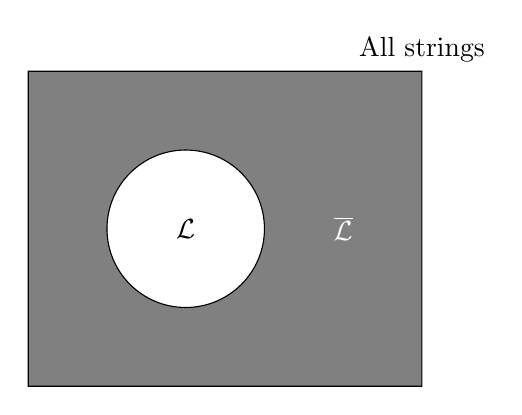
\begin{tikzpicture}[fill=gray]
    \scope
      \clip (-2, -2) rectangle (3, 2)
            (0, 0) circle (1);
      \fill (-2, -2) rectangle (3, 2);
    \endscope
    \scope
      \clip (-2, -2) rectangle (3, 2)
            (0, 0) circle (1);
      \fill (0, 0) circle (1);
    \endscope
    \draw (0, 0) circle (1) (0, 0) node [text = black] {$\mathcal L$}
          (2, 0) node [text = white] {$\overline{\mathcal L}$}
          (-2, -2) rectangle (3, 2) node [text = black, above] {All strings};
  \end{tikzpicture}
\end{center}

\begin{defn}
  The {\boldmath \bfseries complement}  of the language $\mathcal L$ is 
  \[
    \overline{\mathcal L} = \left \{ w : w \not \in \mathcal L \right \}.
  \]
\end{defn}

\begin{thm}
  If $\mathcal L$ is regular then $\overline{\mathcal L}$ is regular.
  In other words, regular languages are closed under complement.
\end{thm}

\begin{prf}
  Swap the accept and reject states of the DFA for $\mathcal L$ to get a DFA for $\overline{\mathcal L}$.

  Formally, if DFA $(Q, \Sigma, \delta, q_0, F)$ recognizes $\mathcal L$ then DFA $(Q, \Sigma, \delta, q_0, Q \setminus F)$ recognizes $\overline{\mathcal L}$.
\end{prf}

\begin{eg}
  $\mathcal L = \left \{ w : w \neq \verb~0~, \verb~1~ \right \}$.
  
  Note that $\overline{\mathcal L} = \left \{ w : w = \verb~0~ \lor w = \verb~1~ \right \}$.
  The DFA for $\overline{\mathcal L}$ is given by: 

  \begin{center}
    \begin{tikzpicture}[> = stealth, node distance = 3em]
      \node[initial, initial text=, state, minimum size = 2em] (0) {};
      \node[right = of 0, accepting, state, minimum size = 2em] (1) {};
      \node[right = of 1, state, minimum size = 2em] (2) {};
      \draw[->]
      (0) edge[above] node{\verb~0~,\verb~1~} (1)
      (1) edge[above] node{\verb~0~,\verb~1~} (2)
      (2) edge[loop right] node{\verb~0~,\verb~1~} (2)
      ;
    \end{tikzpicture}
  \end{center}
  
  Then the DFA for $\mathcal L$ is given by 

  \begin{center}
    \begin{tikzpicture}[> = stealth, node distance = 3em]
      \node[accepting, initial, initial text=, state, minimum size = 2em] (0) {};
      \node[right = of 0, state, minimum size = 2em] (1) {};
      \node[accepting, right = of 1, state, minimum size = 2em] (2) {};
      \draw[->]
      (0) edge[above] node{\verb~0~,\verb~1~} (1)
      (1) edge[above] node{\verb~0~,\verb~1~} (2)
      (2) edge[loop right] node{\verb~0~,\verb~1~} (2)
      ;
    \end{tikzpicture}
  \end{center}
\end{eg}

\begin{eg}
  $\mathcal L = \left \{ w : \text{$w$ does not contain \verb~0101~} \right \}$.
  
  Note that $\overline{\mathcal L} = \left \{ w : \text{$w$ contains \verb~0101~} \right \}$.
  The DFA for $\overline{\mathcal L}$ is given by: 

  \begin{center}
    \begin{tikzpicture}[> = stealth, node distance = 3em]
      \node[initial, initial text=, state, minimum size = 2em] (0) {};
      \node[right = of 0, state, minimum size = 2em] (1) {};
      \node[right = of 1, state, minimum size = 2em] (2) {};
      \node[right = of 2, state, minimum size = 2em] (3) {};
      \node[accepting, right = of 3, state, minimum size = 2em] (4) {};
      \draw[->]
      (0) edge[loop below] node{\verb~1~} (0)
      (0) edge[above] node{\verb~0~} (1)
      (1) edge[loop below] node{\verb~0~} (1)
      (1) edge[above] node{\verb~1~} (2)
      (2) edge[above] node{\verb~0~} (3)
      (2) edge[bend right, above] node{\verb~1~} (0)
      (3) edge[above] node{\verb~1~} (4)
      (3) edge[bend right, above] node{\verb~0~} (1)
      (4) edge[loop below] node{\verb~0~,\verb~1~} (4)
      ;
    \end{tikzpicture}
  \end{center}
  
  Then the DFA for $\mathcal L$ is given by 

  \begin{center}
    \begin{tikzpicture}[> = stealth, node distance = 3em]
      \node[accepting, initial, initial text=, state, minimum size = 2em] (0) {};
      \node[accepting, right = of 0, state, minimum size = 2em] (1) {};
      \node[accepting, right = of 1, state, minimum size = 2em] (2) {};
      \node[accepting, right = of 2, state, minimum size = 2em] (3) {};
      \node[right = of 3, state, minimum size = 2em] (4) {};
      \draw[->]
      (0) edge[loop below] node{\verb~1~} (0)
      (0) edge[above] node{\verb~0~} (1)
      (1) edge[loop below] node{\verb~0~} (1)
      (1) edge[above] node{\verb~1~} (2)
      (2) edge[above] node{\verb~0~} (3)
      (2) edge[bend right, above] node{\verb~1~} (0)
      (3) edge[above] node{\verb~1~} (4)
      (3) edge[bend right, above] node{\verb~0~} (1)
      (4) edge[loop below] node{\verb~0~,\verb~1~} (4)
      ;
    \end{tikzpicture}
  \end{center}
\end{eg}

\subsection{Union and intersection}

\begin{minipage}{0.5 \textwidth}
  \begin{center}
    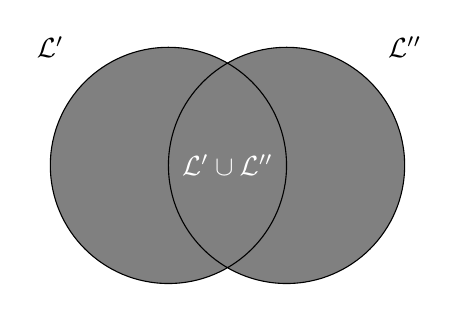
\begin{tikzpicture}[fill=gray]
      \fill (0, 0) circle (1.5);
      \fill (1.5, 0) circle (1.5);
      \draw (0, 0) circle (1.5) (-1.5, 1.5) node[text = black]{$\mathcal L'$}
            (1.5, 0) circle (1.5) (3, 1.5) node[text = black] {$\mathcal L''$}
            (0.75, 0) node[text = white]{$\mathcal L' \cup \mathcal L''$};
    \end{tikzpicture}
  \end{center}
\end{minipage}%
\begin{minipage}{0.5 \textwidth}
  \begin{center}
    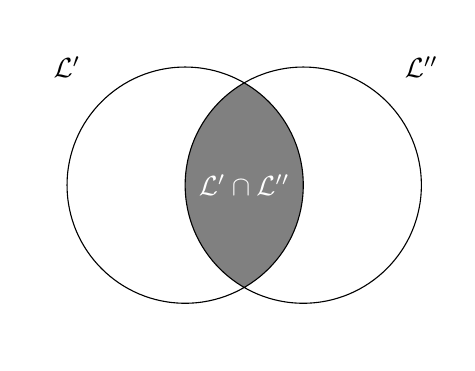
\begin{tikzpicture}[fill=gray]
      \scope
        \clip (-2, -2) rectangle (3, 2)
              (1.5, 0) circle (1.5)
              (0, 0) circle (1.5);
        \fill (0, 0) circle (1.5);
      \endscope
      \draw (0, 0) circle (1.5) (-1.5, 1.5) node[text = black]{$\mathcal L'$}
            (1.5, 0) circle (1.5) (3, 1.5) node[text = black] {$\mathcal L''$}
            (0.75, 0) node[text = white]{$\mathcal L' \cap \mathcal L''$};
    \end{tikzpicture}
  \end{center}
\end{minipage}

\begin{defn}
  The {\boldmath \bfseries union} of languages $\mathcal L'$ and $\mathcal L''$ is 
  \[
    \mathcal L' \cup \mathcal L'' = \left \{ w : w \in \mathcal L' \lor w \in \mathcal L'' \right \}.
  \]
\end{defn}

\begin{defn}
  The {\boldmath \bfseries intersection} of languages $\mathcal L'$ and $\mathcal L''$ is 
  \[
    \mathcal L' \cap \mathcal L'' = \left \{ w : w \in \mathcal L' \land w \in \mathcal L'' \right \}.
  \]
\end{defn}

\begin{thm}
  If $\mathcal L'$, $\mathcal L''$ are regular, then so are 
  \begin{oldenumerate}[topsep = 0ex, label = {(\alph*)}]
    \item $\mathcal L' \cup \mathcal L''$ and 

    \item $\mathcal L' \cap \mathcal L''$.
  \end{oldenumerate}
  
  In other words, regular lanaguages are closed under union and intersection.
\end{thm}

\begin{prf}
  \begin{oldenumerate}[topsep = 0ex, label = {(\alph*)}]
    \item Connect an initial state to the initial states for the NFAs for $\mathcal L'$ and $\mathcal L''$ via $\varepsilon$.
      
    \item If $\mathcal L'$ and $\mathcal L''$ are regular then $\overline{\mathcal L'}$ and $\overline{\mathcal L''}$ are regular.
    Then $\overline{\mathcal L'} \cup \overline{\mathcal L''}$ is regular.
    Then, by De Morgan's law, $\mathcal L' \cap \mathcal L'' = \overline{\overline{\mathcal L'} \cup \overline{\mathcal L''}}$ is regular.
  \end{oldenumerate}
\end{prf}

\begin{prf}
  {\boldmath \bfseries Idea: }\footnote{Here ``E'' stands for ``EVEN'', ``O'' stands for ``ODD'', ``H'' stands for ``HAPPY'', ``W'' stands for ``WORRIED'', and ``S'' stands for ``SAD''.}
  
  \begin{minipage}{0.48 \textwidth}
    \begin{center}
      $\mathcal L' = \left \{ w : \text{$w$ has an even number of \verb~0~s} \right \}$.
    \end{center}
  \end{minipage}%
  \hfill%
  \begin{minipage}{0.48 \textwidth}
    \begin{center}
      $\mathcal L'' = \left \{ w : \text{every \verb~0~ is immediately followed by a \verb~1~} \right \}$.
    \end{center}
  \end{minipage}
  \vspace{0.5 \baselineskip}

  \begin{minipage}{0.45 \textwidth}
    \begin{center}
      \begin{tikzpicture}[> = stealth, node distance = 3em]
        \node[accepting, initial, initial text=, state, minimum size = 2em] (e) {E};
        \node[below = of e, state, minimum size = 2em] (o) {O};
        \draw[->]
        (e) edge[bend right, left] node{\verb~0~} (o)
        (e) edge[loop right] node{\verb~1~} (e)
        (o) edge[bend right, right] node{\verb~0~} (e)
        (o) edge[loop right] node{\verb~1~} (o)
        ;
      \end{tikzpicture}
    \end{center}
  \end{minipage}%
  \hfill%
  \begin{minipage}{0.45 \textwidth}
    \begin{center}
      \begin{tikzpicture}[> = stealth, node distance = 3em]
        \node[accepting, initial, initial text=, state, minimum size = 2em] (h) {H};
        \node[right = of h, state, minimum size = 2em] (w) {W};
        \node[right = of w, state, minimum size = 2em] (s) {S};
        \draw[->]
        (h) edge[loop above] node{\verb~1~} (h)
        (h) edge[bend right, below] node{\verb~0~} (w)
        (w) edge[bend right, above] node{\verb~1~} (h)
        (w) edge[above] node{\verb~0~} (s)
        (s) edge[loop above] node{\verb~0~,\verb~1~} (s)
        ;
      \end{tikzpicture}
    \end{center}
  \end{minipage}
  \vspace{0.5 \baselineskip}
  
  Consider the construction: 

  \begin{center}
    \begin{tikzpicture}[> = stealth, node distance = 3em]
      \node[initial below, initial text=, state, minimum size = 2em] (eh) {E, H};
      \node[right = of eh, state, minimum size = 2em] (ew) {E, W};
      \node[right = of ew, state, minimum size = 2em] (es) {E, S};
      \node[below = of eh, state, minimum size = 2em] (oh) {O, H};
      \node[right = of oh, , state, minimum size = 2em] (ow) {O, W};
      \node[right = of ow, state, minimum size = 2em] (os) {O, S};
      \draw[->]
      (eh) edge[loop left] node{\verb~1~} (eh)
      (eh) edge[] node[above left = 0 and 0.3, sloped]{\verb~0~} (ow)
      (ew) edge[above] node{\verb~1~} (eh)
      (ew) edge[] node[above left = 0 and 0.3, sloped]{\verb~0~} (os)
      (es) edge[loop right] node{\verb~1~} (es)
      (es) edge[bend right, left] node{\verb~0~} (os)
      (oh) edge[loop left] node{\verb~1~} (oh)
      (oh) edge[] node[above left = 0 and 0.3, sloped]{\verb~0~} (ew)
      (ow) edge[above] node{\verb~1~} (oh)
      (ow) edge[] node[above left = 0 and 0.3,  sloped]{\verb~0~} (es)
      (os) edge[loop right] node{\verb~0~} (os)
      (os) edge[bend right, right] node{\verb~0~} (es)
      ;
    \end{tikzpicture}
  \end{center}

  Note that we can create DFAs for either union or intersection by assigning appropriate accept states: 

  \begin{minipage}{0.45 \textwidth}
    \begin{center}
      $\mathcal L = \mathcal L' \cup \mathcal L''.$
    \end{center}
  \end{minipage}%
  \hfill%
  \begin{minipage}{0.45 \textwidth}
    \begin{center}
      $\mathcal L = \mathcal L' \cap \mathcal L''.$
    \end{center}
  \end{minipage}
  \vspace{0.5 \baselineskip}

  \begin{minipage}{0.45 \textwidth}
    \begin{center}
      \scalebox{0.8}{
        \begin{tikzpicture}[> = stealth, node distance = 3em]
          \node[accepting, initial below, initial text=, state, minimum size = 2em] (eh) {E, H};
          \node[accepting, right = of eh, state, minimum size = 2em] (ew) {E, W};
          \node[accepting, right = of ew, state, minimum size = 2em] (es) {E, S};
          \node[accepting, below = of eh, state, minimum size = 2em] (oh) {O, H};
          \node[right = of oh, , state, minimum size = 2em] (ow) {O, W};
          \node[right = of ow, state, minimum size = 2em] (os) {O, S};
          \draw[->]
          (eh) edge[loop left] node{\verb~1~} (eh)
          (eh) edge[] node[above left = 0 and 0.3, sloped]{\verb~0~} (ow)
          (ew) edge[above] node{\verb~1~} (eh)
          (ew) edge[] node[above left = 0 and 0.3, sloped]{\verb~0~} (os)
          (es) edge[loop right] node{\verb~1~} (es)
          (es) edge[bend right, left] node{\verb~0~} (os)
          (oh) edge[loop left] node{\verb~1~} (oh)
          (oh) edge[] node[above left = 0 and 0.3, sloped]{\verb~0~} (ew)
          (ow) edge[above] node{\verb~1~} (oh)
          (ow) edge[] node[above left = 0 and 0.3,  sloped]{\verb~0~} (es)
          (os) edge[loop right] node{\verb~0~} (os)
          (os) edge[bend right, right] node{\verb~0~} (es)
          ;
        \end{tikzpicture}
      }
    \end{center}
  \end{minipage}%
  \hfill%
  \begin{minipage}{0.45 \textwidth}
    \begin{center}
      \scalebox{0.8}{
        \begin{tikzpicture}[> = stealth, node distance = 3em]
          \node[accepting, initial below, initial text=, state, minimum size = 2em] (eh) {E, H};
          \node[right = of eh, state, minimum size = 2em] (ew) {E, W};
          \node[right = of ew, state, minimum size = 2em] (es) {E, S};
          \node[below = of eh, state, minimum size = 2em] (oh) {O, H};
          \node[right = of oh, , state, minimum size = 2em] (ow) {O, W};
          \node[right = of ow, state, minimum size = 2em] (os) {O, S};
          \draw[->]
          (eh) edge[loop left] node{\verb~1~} (eh)
          (eh) edge[] node[above left = 0 and 0.3, sloped]{\verb~0~} (ow)
          (ew) edge[above] node{\verb~1~} (eh)
          (ew) edge[] node[above left = 0 and 0.3, sloped]{\verb~0~} (os)
          (es) edge[loop right] node{\verb~1~} (es)
          (es) edge[bend right, left] node{\verb~0~} (os)
          (oh) edge[loop left] node{\verb~1~} (oh)
          (oh) edge[] node[above left = 0 and 0.3, sloped]{\verb~0~} (ew)
          (ow) edge[above] node{\verb~1~} (oh)
          (ow) edge[] node[above left = 0 and 0.3,  sloped]{\verb~0~} (es)
          (os) edge[loop right] node{\verb~0~} (os)
          (os) edge[bend right, right] node{\verb~0~} (es)
          ;
        \end{tikzpicture}
      }
    \end{center}
  \end{minipage}
  \vspace{0.5 \baselineskip}
  
  Note that this construction is better than that in the first proof since the number of nodes in this construction is $\mathcal O(n^2)$ while that in the first proof is $\mathcal O(4^n)$.
  
  Formally, write the DFA for $\mathcal L'$ as $(Q', \Sigma, \delta', q_0', F')$ and that for $\mathcal L''$ as $(Q'', \Sigma, \delta'', q_0'', F'')$.
  
  Then the DFA for $\mathcal L' \cup \mathcal L''$ is given by $(Q' \times Q'', \Sigma, \delta, (q_0', q_0''), (F' \times Q'') \cup (Q' \times F''))$ where $\delta((q', q''), \sigma) := (\delta'(q', \sigma), \delta''(q'', \delta))$ for all $q' \in Q'$, $q'' \in Q''$, and $\sigma \in \Sigma$.

  Similarly, the DFA for $\mathcal L' \cap \mathcal L''$ is given by $(Q' \times Q'', \Sigma, \delta, (q_0', q_0''), F' \times F'')$ where \\ $\delta((q', q''), \sigma) := (\delta'(q', \sigma), \delta''(q'', \delta))$ for all $q' \in Q'$, $q'' \in Q''$, and $\sigma \in \Sigma$.
\end{prf}

\begin{cor}
  If $\mathcal L_1, \mathcal L_2, \dots, \mathcal L_n$ are regular, so are 
  \begin{itemize}
    \item $\mathcal L_1 \cup \mathcal L_2 \cup \cdots \cup \mathcal L_n$ and 

    \item $\mathcal L_1 \cap \mathcal L_2 \cap \cdots \cap \mathcal L_n$.
  \end{itemize}
\end{cor}

\begin{prf}
  Induction.
\end{prf}

\begin{cor}
  Every finite language is regular.
\end{cor}

\begin{prf}
  Let $\mathcal L$ be finite.
  Then we can write 
  \[
    \mathcal L = \bigcup_{w \in \mathcal L} \left \{ w \right \}, 
  \]
  that is, as a union of singleton languages.

  Note that an NFA can be easily found for any singleton language, that is, singleton languages are regular.
  Then $\mathcal L$ is regular by Corollary~\ref{cor:4.2.4}.
\end{prf}

\newpage

\subsection{Difference}

\begin{center}
  $\mathcal L' \setminus \mathcal L'' = \left \{ w \in \mathcal L' : w \not \in \mathcal L'' \right \}$
\end{center}

\begin{center}
  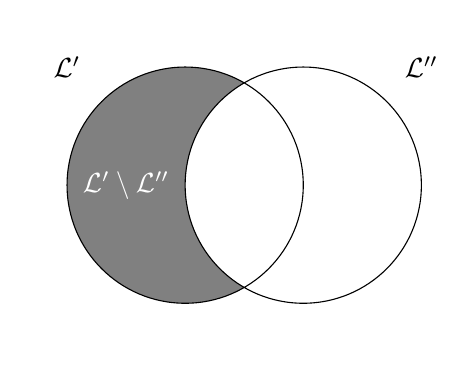
\begin{tikzpicture}[fill=gray]
    \scope
      \clip (-2, -2) rectangle (3, 2)
            (1.5, 0) circle (1.5);
      \fill (0, 0) circle (1.5);
    \endscope
    \draw (0, 0) circle (1.5) (-1.5, 1.5) node[text = black]{$\mathcal L'$}
          (1.5, 0) circle (1.5) (3, 1.5) node[text = black] {$\mathcal L''$}
          (-0.75, 0) node[text = white]{$\mathcal L' \setminus \mathcal L''$};
  \end{tikzpicture}
\end{center}

\begin{thm}
  If $\mathcal L'$ and $\mathcal L''$ are regular then so is $\mathcal L' \setminus \mathcal L''$.
\end{thm}

\begin{prf}
  $\mathcal L' \setminus \mathcal L'' = \mathcal L' \cap \overline{\mathcal L''}$.
\end{prf}

\begin{cor}
  If $\mathcal A$, $\mathcal S$ are regular, then so is $\mathcal L = \left \{ w \in \mathcal A : \text{no substring of $w$ is in $\mathcal S$} \right \}$.
\end{cor}

\begin{prf}
  Let $\mathcal S' = \left \{ w : \text{some substring of $w$ is in $\mathcal S$} \right \}$.
  Note that $\mathcal S'$ is a superset of $\mathcal S$.
  An NFA for $\mathcal S'$ is given by: 
  
  \begin{center}
    \begin{tikzpicture}[> = stealth, node distance = 3em]
      \node[initial, initial text=, state, minimum size = 2em] (x) {};
      \node[right = of x, style = {draw, rectangle, minimum width = 4em, minimum height = 2em}, minimum size = 2em] (nfa) {NFA for $\mathcal S$};
      \draw[->]
      (x) edge[loop above] node{\verb~0~,\verb~1~} (x)
      (x) edge[above] node{$\varepsilon$} (nfa)
      (nfa) edge[loop above] node{\verb~0~,\verb~1~} (nfa)
      ;
    \end{tikzpicture}
  \end{center}
  where the self loop on NFA for $\mathcal S$ refers to self loops on the accept states of the NFA.
  
  Since $\mathcal S'$ is regular by construction, $\mathcal L = \mathcal A \setminus \mathcal S'$ is regular.
\end{prf}

\subsection{Concatenation}

\begin{defn}
  The {\boldmath \bfseries concatenation} of two languages $\mathcal L'$ and $\mathcal L''$, is given by 
  \[
    \mathcal L' \mathcal L'' = \left \{ w' w'' : w' \in \mathcal L' \quad \land \quad w'' \in \mathcal L'' \right \}.
  \]
  
  This is sometimes denoted as $\mathcal L' \circ \mathcal L''$.
\end{defn}

\begin{eg}
  Given $\mathcal L' = \left \{ \verb~000~, \verb~111~ \right \}$ and $\mathcal L'' = \left \{ \verb~10~, \verb~010~ \right \}$, we have 
  \[
    \mathcal L' \mathcal L'' = \left \{ \verb~00010~, \verb~000010~, \verb~11110~, \verb~111010~ \right \}.
  \]
\end{eg}

{\boldmath \bfseries Observation: } $\mathcal L \varnothing \varnothing \mathcal L = \varnothing$ and $\mathcal L \left \{ \varepsilon \right \} = \left \{ \varepsilon \right \} \mathcal L = \mathcal L$ for any language $\mathcal L$.

\begin{thm}
  If $\mathcal L'$ and $\mathcal L''$ are regular then so is $\mathcal L' \mathcal L''.$
\end{thm}

\begin{prf}
  An NFA for $\mathcal L' \mathcal L''$ is given by: 
  
  \begin{center}
    \begin{tikzpicture}[> = stealth, node distance = 3em]
      \node[initial, initial text=, style = {draw, rectangle, minimum width = 4em, minimum height = 2em}, minimum size = 2em] (nfa1) {NFA for $\mathcal L'$};
      \node[right = of nfa1, style = {draw, rectangle, minimum width = 4em, minimum height = 2em}, minimum size = 2em] (nfa2) {NFA for $\mathcal L''$};
      \draw[->]
      (nfa1) edge[above] node{$\varepsilon$} (nfa2)
      ;
    \end{tikzpicture}
  \end{center}
  where the $\varepsilon$ transition from the first NFA to the second NFA refer to those from the accept states in the first NFA to the start state of the second and all accept states in the first NFA are converted to reject states.

  Formally, write the first NFA as $(Q', \Sigma, \delta', q'_0, F')$ and the second NFA as $(Q'', \Sigma, \delta', q''_0, F'')$.
  Then we 
  \begin{itemize}
    \item make every state in $F'$ a reject state and

    \item add $\varepsilon$ transitions from every state in $F'$ to $q''_0$.
  \end{itemize}
\end{prf}

\begin{eg}
  An NFA for $\left \{ u w : \text{$\left | u \right |$ is odd, $v$ contains at least two \verb~0~s} \right \}$ is given by: 

  \begin{center}
    \begin{tikzpicture}[> = stealth, node distance = 3em]
      \node[initial, initial text=, state, minimum size = 2em] (0) {};
      \node[right = of 0, state, minimum size = 2em] (1) {};
      \node[right = of 1, state, minimum size = 2em] (2) {};
      \node[right = of 2, state, minimum size = 2em] (3) {};
      \node[accepting, right = of 3, state, minimum size = 2em] (4) {};
      \draw[->]
      (0) edge[bend right, below] node{\verb~0~,\verb~1~} (1)
      (1) edge[bend right, above] node{\verb~0~,\verb~1~} (0)
      (1) edge[above] node{$\varepsilon$} (2)
      (2) edge[loop above] node{\verb~1~} (2)
      (2) edge[above] node{\verb~0~} (3)
      (3) edge[loop above] node{\verb~1~} (3)
      (3) edge[above] node{\verb~0~} (4)
      (4) edge[loop above] node{\verb~0~,\verb~1~} (4)
      ;
    \end{tikzpicture}
  \end{center}
\end{eg}

\subsection{Kleene star}

\begin{defn}
  The {\boldmath \bfseries Kleene star} of a language $\mathcal L$ is given by 
  \[
    \mathcal L^* = \left \{ w : \text{$w$ is the concatenation of zero or more strings in $\mathcal L$} \right \}.
  \]
\end{defn}

\begin{eg}
  The Kleene star of $\mathcal L = \left \{ \verb~a~, \verb~b~ \right \}$ is given by 
  \[
    \mathcal L^* = \left \{ \varepsilon, \verb~a~, \verb~b~, \verb~aa~, \verb~ab~, \verb~ba~, \verb~bb~, \dots \right \}.
  \]
  
  In words, $\left \{ \verb~a~, \verb~b~ \right \}^* = $ the set of all strings over the alphabet $\left \{ \verb~a~, \verb~b~ \right \}$.
\end{eg}

{\boldmath \bfseries Observation: } $\varnothing^* = \left \{ \varepsilon \right \}^* = \left \{ \varepsilon \right \}$.

{\boldmath \bfseries Observation: } $\mathcal L^*$ is finite if and only if $\mathcal L = \varnothing$ or $\mathcal L = \left \{ \varepsilon \right \}$.

\begin{thm}
  If $\mathcal L$ is regular then so is $\mathcal L^*$.
\end{thm}

\begin{prf}
  {\color{red} (Incorrect)} Note that 
  \[
    \mathcal L^* = \left \{ \varepsilon \right \} \cup \mathcal L \cup \mathcal L \mathcal L \cup \cdots \cup \underbrace{\mathcal L \cdots \mathcal L}_{n} \cup \cdots, 
  \]
  and since the union of regular languages is regular, $\mathcal L^*$ is regular.
  
  However, note that the theorem that the union of regular languages is regular does not work for an infinite number of languages and therefore this proof fails.
\end{prf}

\begin{prf}
  {\color{red} (Incorrect)} An NFA for $\mathcal L^*$ is given by 

  \begin{center}
    \begin{tikzpicture}[> = stealth, node distance = 3em]
      \node[initial, initial text=, style = {draw, rectangle, minimum width = 4em, minimum height = 2em}, minimum size = 2em] (nfa) {NFA for $\mathcal L$};
      \draw[->]
      (nfa) edge[loop above] node{$\varepsilon$} (nfa)
      ;
    \end{tikzpicture}
  \end{center}
  where the self loop on the NFA refers to $\varepsilon$ transitions from the accept states of the NFA to the start state and the start state is converted to an accept state.
  
  However, this construction fails if $q_0$ is originally rejecting \textit{and} part of a cycle.
\end{prf}

\begin{prf}
  {\color{green} (Correct)} An NFA for $\mathcal L^*$ is given by 

  \begin{center}
    \begin{tikzpicture}[> = stealth, node distance = 3em]
      \node[accepting, initial, initial text=, state, minimum size = 2em] (s) {};
      \node[right = of s, style = {draw, rectangle, minimum width = 4em, minimum height = 2em}, minimum size = 2em] (nfa) {NFA for $\mathcal L$};
      \draw[->]
      (s) edge[above] node{$\varepsilon$} (nfa)
      (nfa) edge[loop above] node{$\varepsilon$} (nfa)
      ;
    \end{tikzpicture}
  \end{center}
  where the self loop on the NFA refers to $\varepsilon$ transitions from the accept states of the NFA to the start state.
  
  In words, add $\varepsilon$-transitions from every state in $F$ to $q_0$ and add a new start state $q'_0$ and link it with an $\varepsilon$-arrow to $q_0$.
\end{prf}

\subsection{Reverse}

\begin{defn}
  For a string $w = w_1 w_2 \dots w_n$, its {\boldmath \bfseries reverse} is given by 
  \[
    w^R = w_n w_{n - 1} \dots w_2 w_1.
  \]
\end{defn}

\begin{defn}
  The {\boldmath \bfseries reverse} of a language $\mathcal L$ is given by
  \[
    \mathcal L^R = \left \{ w^R : w \in \mathcal L \right \}.
  \]
\end{defn}

\begin{eg}
  $\left \{ \verb~011~, \verb~abc~ \right \}^R = \left \{ \verb~110~, \verb~cba~ \right \}$.
\end{eg}

\begin{thm}
  If $\mathcal L$ is regular then so is $\mathcal L^R$.
\end{thm}

\begin{prf}
  Consider an NFA $(Q, \Sigma, \delta, q_0, F)$ for $\mathcal L$.
  Reverse all the transitions, create a new start state, and link it with $\varepsilon$-transitions to states in $F$.
  Make $q_0$ the only accept state.
\end{prf}

\subsection{Prefix and suffix}

\begin{defn}
  The {\boldmath \bfseries prefix language} of a language $\mathcal L$ is given by 
  \[
    \operatorname{prefix}(\mathcal L) = \left \{ u : u v \in \mathcal L \text{ for some string $v$, possibly empty} \right \}.
  \]
\end{defn}

\begin{defn}
  The {\boldmath \bfseries suffix language} of a language $\mathcal L$ is given by 
  \[
    \operatorname{suffix}(\mathcal L) = \left \{ v : u v \in \mathcal L \text{ for some string $u$, possibly empty} \right \}.
  \]
\end{defn}

\begin{thm}
  If $\mathcal L$ is regular then so is $\operatorname{prefix}(\mathcal L)$.
\end{thm}

\begin{prf}
  Given a DFA $(Q, \Sigma, \delta, q_0, F)$ for $\mathcal L$, a DFA for $\operatorname{prefix}(\mathcal L)$ is given by $(Q, \Sigma, \delta, q_0, F')$ where 
  \[
    F' = \left \{ q \in Q : \text{there exists a path, possibly empty, from $q$ to a state in $F$} \right \}
  \]
\end{prf}

\begin{cor}
  If $\mathcal L$ is regular then so is $\operatorname{suffix}(\mathcal L)$.
\end{cor}

\begin{prf}
  $\operatorname{suffix}(\mathcal L) = (\operatorname{prefix}(\mathcal L^R))^R$.
\end{prf}

\subsection{Substring}

\begin{defn}
  The {\boldmath \bfseries substring language} of a language $\mathcal L$ is given by 
  \[
    \operatorname{substring}(\mathcal L) = \left \{ v : uvw \in \mathcal L \text{ for some strings $u$, $w$} \right \}.
  \]
\end{defn}

\begin{thm}
  If $\mathcal L$ is regular then so is $\operatorname{substring}(\mathcal L)$.
\end{thm}

\begin{prf}
  $\operatorname{substring}(\mathcal L) = \operatorname{suffix}(\operatorname{prefix}(\mathcal L))$.
\end{prf}

\subsection{Shuffle}

\begin{defn}
  The {\boldmath \bfseries shuffle language} of two languages $\mathcal L'$ and $\mathcal L''$ is given by 
  \[
    \left \{ a_1 b_1 a_2 b_2 \dots a_k b_k : a_1, \dots, a_k \text{ strings}, b_1, \dots, b_k \text{ strings}, a_1 \cdots a_k \in \mathcal L', b_1 \cdots b_k \in \mathcal L'' \right \}.
  \]
\end{defn}

\begin{prf}
  Given an NFA $(Q', \Sigma, \delta', q'_0, F')$ for $\mathcal L'$ and an NFA $(Q'', \Sigma, \delta'', q''_0, F'')$ for $\mathcal L''$, an NFA for $\mathcal L' \diamond \mathcal L''$ is given by $(Q' \times Q'', \Sigma, \Delta, (q'_0, q''_0), F' \times F'')$ where 
  \[
    \Delta((q', q''), \sigma) = \left ( \delta'(q', \sigma) \times \left \{ q'' \right \} \right ) \cup \left ( \left \{ q' \right \} \times \delta''(q'', \sigma) \right ).
  \]
\end{prf}

\section{Regular expressions}

\subsection{Basic notions}

\begin{defn}
  A regular expression is 
  \begin{olditemize}[topsep = 0ex, itemsep = 0ex]
    \item $\varnothing$, 

    \item $\left \{ \varepsilon \right \}$, 

    \item $\left \{ \sigma \right \}$ for $\sigma \in \Sigma$, 

    \item $(R^*)$, % BEGIN BRACE

    \item $(R_1 \cup R_2)$, and

    \item $(R_1 \circ R_2)$. % END BRACE - where $R$, $R_1$, $R_2$ are regular expressions
  \end{olditemize}
\end{defn}

\begin{eg}
  $\left ( \left ( \left ( \left \{ \verb~0~ \right \} \cup \left \{ \verb~1~ \right \} \right )^* \right ) \cup \left \{ \verb~1~ \right \} \right )$.
\end{eg}

\begin{eg}
  $\left ( \left ( \left ( \left \{ \verb~0~ \right \} \circ \left \{ \verb~1~ \right \} \right ) \circ \left \{ \verb~1~ \right \} \right ) \circ \left \{ \verb~1~ \right \} \right )$.
\end{eg}

\begin{eg}
  $((((\left \{ \verb~0~ \right \} \circ \left \{ \verb~1~ \right \})^*) \circ \left \{ \verb~1~ \right \}) \circ ((\left \{ \verb~0~ \right \} \cup \left \{ \verb~1~ \right \})^*))$
\end{eg}

{\boldmath \bfseries Shorthand}

\begin{itemize}
  \item $R^k = \underbrace{(R \circ R \circ \cdots \circ R)}_{k}$
    
  \item $R^+ = (R \circ (R^*))$
    
  \item $\Sigma = (\left \{ \verb~0~ \right \} \cup \left \{ \verb~1~ \right \})$ assuming alpha bet is $\left \{ \verb~0~, \verb~1~ \right \}$
    
  \item may omit $\left \{ \right \}$, $()$, $\circ$
\end{itemize}

{\boldmath \bfseries Precedence:} $*$ then $\circ$ then $\cup$.

\begin{note}
  Sometimes $()$ are necessary.
\end{note}

\begin{eg}
  Example~\ref{eg:5.1.2} can be simplified to $\Sigma^* \cup \left \{ 1 \right \} = \Sigma^*$.
\end{eg}

\begin{eg}
  Example~\ref{eg:5.1.3} can be simplified to \verb~0111~.
\end{eg}

\begin{eg}
  Example~\ref{eg:5.1.4} can be simplified to $\Sigma^* \verb~1~ \Sigma^*$.
\end{eg}

\begin{eg}
  A regular expression for $\left \{ w : \text{$w$ contains exactly one \verb~1~} \right \}$ is $\verb~0~^* \verb~1~ \verb~0~^*$.
\end{eg}

\begin{eg}
  A regular expression for $\left \{ w : \text{$w$ contains at least one \verb~1~} \right \}$ is $\Sigma^* \verb~1~ \Sigma^*$.
\end{eg}

\begin{eg}
  A regular expression for $\left \{ w : \text{$w$ contains \verb~001~ as a substring} \right \}$ is $\Sigma^* \verb~001~ \Sigma^*$.
\end{eg}

\begin{eg}
  A regular expression for $\left \{ w : \text{$w$ does not contain \verb~00~ as a substring} \right \}$ is $\verb~1~^* (\verb~0~ \verb~1~^+)^* (\varepsilon \cup \verb~0~)$.
\end{eg}

\begin{eg}
  A regular expression for $\left \{ w : \text{$|w|$ is even} \right \}$ is $(\Sigma^2)^*$.
\end{eg}

\begin{eg}
  A regular expression for $\left \{ w : 5 \mid |w| \right \}$ is $(\Sigma^5)^*$.
\end{eg}

\begin{eg}
  A regular expression for $\left \{ w : w \neq \varepsilon \land w_1 = w_{|w|} \right \}$ is $\Sigma \cup \verb~0~ \Sigma^* \verb~0~ \cup \verb~1~ \Sigma^* \verb~1~$.
\end{eg}

\begin{eg}
  A regular expression for $\left \{ \verb~01~, \verb~10~ \right \}$ is $\verb~01~ \cup \verb~10~$.
\end{eg}

\begin{eg}
  The regular expression $(\verb~0~ \cup \varepsilon) 1^*$ can be arguably simplified to $\verb~01~^* \cup 1^*$.
\end{eg}

\begin{eg}
  The regular expression $\verb~1~^* \varnothing$ can be simplified to $\varnothing$.
\end{eg}

\begin{eg}
  The regular expression $\varnothing^*$ can be simplified to $\varepsilon$.
\end{eg}

\begin{eg}
  The regular expression $(\verb~0~ \cup \verb~1~^+ \verb~0~)^*$ can be simplified to $((\varepsilon \cup \verb~1~^+) \verb~0~)*$ and then to $(\verb~1~^* \verb~0~)^*$.
  In words, all strings that do not end in a \verb~1~.
\end{eg}

\begin{eg}
  \begin{center}
    \begin{tabular}{c|c|c}
      Regular expression & Shortest accepted string & Shortest rejected string \\ 
      \hline
      $\verb~0~^* \verb~0011~^*$ & \verb~001~ & $\varepsilon$ \\ 
      $\verb~0~^* \verb~00~ (\verb~0~ \cup \verb~1~)^*$ & \verb~00~ & $\varepsilon$ \\ 
      $(\verb~00~)^* (\verb~110~)^* (\verb~11~)^*$ & $\varepsilon$ & \verb~0~, \verb~1~ \\ 
      $\verb~0~^* (\verb~01~ \cup \verb~10~)^* \verb~1~^*$ & $\varepsilon$ & \verb~100~, \verb~110~
    \end{tabular}
  \end{center}
\end{eg}

\subsection{Equivalence with automata}

\begin{thm}
  The language of every regular expression is regular.
\end{thm}

\begin{prf}
  Induction.
\end{prf}

\begin{thm}[Kleene's theorem]
  Then language of every NFA can be represented by a regular expression.
\end{thm}

\begin{prf}
  Given an NFA, create a new state state and a new and unique accept state (making every state in the original NFA rejecting).
  Choose a state other than the start state and the accept state.
  Call the states from which the incoming transitions originate donors and those at which the outgoing transitions arrive receivers.
  Note that a state can be both a donor and a receiver.
  Then for each donor-receiver pair, replace the transitions with a single transition $\alpha \beta^* \gamma$ where $\alpha$ is the incoming transition, $\beta$ is the looping transition, and $\gamma$ is the outgoing transition.
  Remove the chosen state.
  Collapse any parallel edges created in the process by unioning them.
  If there are states other than the start state or the accept state, repeat the process.
  If there are no transitions from the start state to the accept state then the regular expression is $\varnothing$.
  Otherwise there is exactly one transition $\alpha$, the desired regular expression.
\end{prf}

\subsection{Conversion example}

\begin{center}
  \begin{tikzpicture}[> = stealth, node distance = 3em]
    \node[initial, initial text=, state, minimum size = 2em] (0) {};
    \node[right = of 0, accepting, state, minimum size = 2em] (1) {};
    \node[right = of 1, state, minimum size = 2em] (2) {};
    \node[accepting, right = of 2, state, minimum size = 2em] (3) {};
    \node[below = of 0, state, minimum size = 2em] (4) {};
    \draw[->]
    (0) edge[above] node{\verb~0~,\verb~1~} (1)
    (0) edge[left] node{\verb~0~} (4)
    (1) edge[bend right = 15, above left] node{\verb~0~} (4)
    (1) edge[above] node{\verb~1~} (2)
    (2) edge[loop below] node{\verb~0~} (2)
    (2) edge[above] node{\verb~1~} (3)
    (4) edge[bend right = 15, below right] node{\verb~1~} (1)
    ;
  \end{tikzpicture}
\end{center}

\begin{center}
  \begin{tikzpicture}[> = stealth, node distance = 3em]
    \node[color = red, initial, initial text=, state, minimum size = 2em] (s) {};
    \node[right = of s, state, minimum size = 2em] (0) {};
    \node[right = of 0, color = red, state, minimum size = 2em] (1) {};
    \node[right = of 1, state, minimum size = 2em] (2) {};
    \node[color = red, right = of 2, state, minimum size = 2em] (3) {};
    \node[below = of 0, state, minimum size = 2em] (4) {};
    \node[color = red, accepting, right = of 3, state, minimum size = 2em] (e) {};
    \draw[->]
    (s) edge[color = red, above] node{$\varepsilon$} (0)
    (0) edge[above] node{\verb~0~,\verb~1~} (1)
    (0) edge[left] node{\verb~0~} (4)
    (1) edge[bend right = 15, above left] node{\verb~0~} (4)
    (1) edge[above] node{\verb~1~} (2)
    (1) edge[bend left = 40, above, color = red] node{$\varepsilon$} (e)
    (2) edge[loop below] node{\verb~0~} (2)
    (2) edge[above] node{\verb~1~} (3)
    (3) edge[color = red, above] node{$\varepsilon$} (e)
    (4) edge[bend right = 15, below right] node{\verb~1~} (1)
    ;
  \end{tikzpicture}
\end{center}

\begin{center}
  \begin{tikzpicture}[> = stealth, node distance = 3em]
    \node[initial, initial text=, state, minimum size = 2em] (s) {};
    \node[right = of s, state, minimum size = 2em] (0) {};
    \node[right = of 0, state, minimum size = 2em] (1) {};
    \node[right = of 1, minimum size = 2em] (2) {};
    \node[right = of 2, state, minimum size = 2em] (3) {};
    \node[below = of 0, state, minimum size = 2em] (4) {};
    \node[accepting, right = of 3, state, minimum size = 2em] (e) {};
    \draw[->]
    (s) edge[above] node{$\varepsilon$} (0)
    (0) edge[above] node{\verb~0~,\verb~1~} (1)
    (0) edge[left] node{\verb~0~} (4)
    (1) edge[bend right = 15, above left] node{\verb~0~} (4)
    (1) edge[bend left = 40, above] node{$\varepsilon$} (e)
    (1) edge[color = red, above] node{$\verb~10~^* \verb~1~$} (3)
    (3) edge[above] node{$\varepsilon$} (e)
    (4) edge[bend right = 15, below right] node{\verb~1~} (1)
    ;
  \end{tikzpicture}
\end{center}

\begin{center}
  \begin{tikzpicture}[> = stealth, node distance = 3em]
    \node[initial, initial text=, state, minimum size = 2em] (s) {};
    \node[right = of s, state, minimum size = 2em] (0) {};
    \node[right = of 0, state, minimum size = 2em] (1) {};
    \node[right = of 1, minimum size = 2em] (2) {};
    \node[right = of 2, minimum size = 2em] (3) {};
    \node[below = of 0, state, minimum size = 2em] (4) {};
    \node[accepting, right = of 3, state, minimum size = 2em] (e) {};
    \draw[->]
    (s) edge[above] node{$\varepsilon$} (0)
    (0) edge[above] node{\verb~0~,\verb~1~} (1)
    (0) edge[left] node{\verb~0~} (4)
    (1) edge[bend right = 15, above left] node{\verb~0~} (4)
    (1) edge[color = red, above] node{$\verb~10~^* \verb~1~ \cup \varepsilon$} (e)
    (4) edge[bend right = 15, below right] node{\verb~1~} (1)
    ;
  \end{tikzpicture}
\end{center}

\begin{center}
  \begin{tikzpicture}[> = stealth, node distance = 3em]
    \node[initial, initial text=, state, minimum size = 2em] (s) {};
    \node[right = of s, minimum size = 2em] (0) {};
    \node[right = of 0, state, minimum size = 2em] (1) {};
    \node[right = of 1, minimum size = 2em] (2) {};
    \node[right = of 2, minimum size = 2em] (3) {};
    \node[below = of 0, state, minimum size = 2em] (4) {};
    \node[accepting, right = of 3, state, minimum size = 2em] (e) {};
    \draw[->]
    (s) edge[color = red, above] node{$\Sigma$} (1)
    (s) edge[color = red, below left] node{\verb~0~} (4)
    (1) edge[bend right = 15, above left] node{\verb~0~} (4)
    (1) edge[above] node{$\verb~10~^* \verb~1~ \cup \varepsilon$} (e)
    (4) edge[bend right = 15, below right] node{\verb~1~} (1)
    ;
  \end{tikzpicture}
\end{center}

\begin{center}
  \begin{tikzpicture}[> = stealth, node distance = 3em]
    \node[initial, initial text=, state, minimum size = 2em] (s) {};
    \node[right = of s, minimum size = 2em] (0) {};
    \node[right = of 0, state, minimum size = 2em] (1) {};
    \node[right = of 1, minimum size = 2em] (2) {};
    \node[right = of 2, minimum size = 2em] (3) {};
    \node[below = of 0, minimum size = 2em] (4) {};
    \node[accepting, right = of 3, state, minimum size = 2em] (e) {};
    \draw[->]
    (s) edge[color = red, above] node{$\Sigma \cup \verb~01~$} (1)
    (1) edge[color = red, loop above] node{\verb~01~} (1)
    (1) edge[above] node{$\verb~10~^* \verb~1~ \cup \varepsilon$} (e)
    ;
  \end{tikzpicture}
\end{center}

\begin{center}
  \begin{tikzpicture}[> = stealth, node distance = 3em]
    \node[initial, initial text=, state, minimum size = 2em] (s) {};
    \node[right = of s, minimum size = 2em] (0) {};
    \node[right = of 0, minimum size = 2em] (1) {};
    \node[right = of 1, minimum size = 2em] (2) {};
    \node[right = of 2, minimum size = 2em] (3) {};
    \node[below = of 0, minimum size = 2em] (4) {};
    \node[accepting, right = of 3, state, minimum size = 2em] (e) {};
    \draw[->]
    (s) edge[color = red, above] node{$(\Sigma \cup \verb~01~) (\verb~01~)^* (\verb~10~^* \verb~1~ \cup \varepsilon)$} (e)
    ;
  \end{tikzpicture}
\end{center}

\subsection{Conversion example \#2}

\begin{center}
  \begin{tikzpicture}[> = stealth, node distance = 5em]
    \node[accepting, initial, initial text=, state, minimum size = 2em] (0) {};
    \node[above right = of 0, state, minimum size = 2em] (1) {};
    \node[below right = of 0, state, minimum size = 2em] (2) {};
    \node[above right = of 2, state, minimum size = 2em] (3) {};
    \node[right = of 3, state, minimum size = 2em] (4) {};
    \draw[->]
    (0) edge[above left] node{\verb~0~} (1)
    (0) edge[bend right = 15, below left] node{\verb~1~} (2)
    (1) edge[bend right = 15, left] node{\verb~1~} (2)
    (2) edge[bend right = 15, above] node{\verb~1~} (0)
    (2) edge[bend right = 15, right] node{\verb~0~} (1)
    (0) edge[loop above] node{\verb~1~} (0)
    (0) edge[bend right = 85, looseness = 3.5, below] node{\verb~1~} (3)
    (3) edge[above right] node{\verb~0~} (1)
    (2) edge[below right] node{\verb~1~} (3)
    (4) edge[loop below] node{\verb~0~,\verb~1~} (4)
    (4) edge[bend right, above] node{\verb~0~} (1)
    (4) edge[above] node{\verb~0~} (3)
    (2) edge[loop below] node{\verb~1~} (2)
    ;
  \end{tikzpicture}
\end{center}

\begin{center}
  \begin{tikzpicture}[> = stealth, node distance = 5em]
    \node[initial, initial text=, color = red, state, minimum size = 2em] (s) {};
    \node[right = of s, color = red, state, minimum size = 2em] (0) {};
    \node[above right = of 0, state, minimum size = 2em] (1) {};
    \node[below right = of 0, state, minimum size = 2em] (2) {};
    \node[above right = of 2, state, minimum size = 2em] (3) {};
    \node[accepting, below = of s, color = red, state, minimum size = 2em] (e) {};
    \draw[->]
    (s) edge[color = red, above] node{$\varepsilon$} (0)
    (0) edge[color = red, above left] node{$\varepsilon$} (e)
    (0) edge[bend right = 15, below left] node{\verb~1~} (2)
    (0) edge[above left] node{\verb~0~} (1)
    (1) edge[bend right = 15, left] node{\verb~1~} (2)
    (2) edge[bend right = 15, above] node{\verb~1~} (0)
    (2) edge[bend right = 15, right] node{\verb~0~} (1)
    (0) edge[loop above] node{\verb~1~} (0)
    (0) edge[bend right = 85, looseness = 3.5, below] node{\verb~1~} (3)
    (3) edge[above right] node{\verb~0~} (1)
    (2) edge[below right] node{\verb~1~} (3)
    (2) edge[loop below] node{\verb~1~} (2)
    ;
  \end{tikzpicture}
\end{center}

\begin{center}
  \begin{tikzpicture}[> = stealth, node distance = 5em]
    \node[initial, initial text=, state, minimum size = 2em] (s) {};
    \node[right = of s, state, minimum size = 2em] (0) {};
    \node[above right = of 0, state, minimum size = 2em] (1) {};
    \node[below right = of 0, state, minimum size = 2em] (2) {};
    \node[accepting, below = of s, state, minimum size = 2em] (e) {};
    \draw[->]
    (s) edge[above] node{$\varepsilon$} (0)
    (0) edge[above left] node{$\varepsilon$} (e)
    (0) edge[color = red, above] node[sloped]{$\verb~0~ \cup \verb~10~$} (1)
    (0) edge[bend right = 15, below left] node{\verb~1~} (2)
    (1) edge[bend right = 15, left] node{\verb~1~} (2)
    (2) edge[bend right = 15, above] node{\verb~1~} (0)
    (2) edge[color = red, bend right = 15, right] node{$\verb~0~ \cup \verb~10~$} (1)
    (0) edge[loop above] node{\verb~1~} (0)
    (2) edge[loop below] node{\verb~1~} (2)
    ;
  \end{tikzpicture}
\end{center}

\begin{center}
  \begin{tikzpicture}[> = stealth, node distance = 5em]
    \node[initial, initial text=, state, minimum size = 2em] (s) {};
    \node[right = of s, state, minimum size = 2em] (0) {};
    \node[below right = of 0, state, minimum size = 2em] (2) {};
    \node[accepting, below = of s, state, minimum size = 2em] (e) {};
    \draw[->]
    (s) edge[above] node{$\varepsilon$} (0)
    (0) edge[above left] node{$\varepsilon$} (e)
    (0) edge[color = red, bend right = 15, below] node[sloped]{$\verb~1~ \cup (\verb~0~ \cup \verb~01~) \verb~1~$} (2)
    (2) edge[bend right = 15, above] node[]{\verb~1~} (0)
    (0) edge[loop above] node{\verb~1~} (0)
    (2) edge[color = red, loop below] node{$\verb~1~ \cup (\verb~0~ \cup \verb~10~) \verb~1~$} (2)
    ;
  \end{tikzpicture}
\end{center}

\begin{center}
  \begin{tikzpicture}[> = stealth, node distance = 5em]
    \node[initial, initial text=, state, minimum size = 2em] (s) {};
    \node[right = of s, state, minimum size = 2em] (0) {};
    \node[accepting, right = of 0, state, minimum size = 2em] (e) {};
    \draw[->]
    (s) edge[above] node{$\varepsilon$} (0)
    (0) edge[above left] node{$\varepsilon$} (e)
    (0) edge[color = red, loop above] node{$\verb~1~ \cup \Big ( 1 \cup (\verb~0~ \cup \verb~10~) \verb~1~ \Big ) \Big ( \verb~1~ \cup (\verb~0~ \cup \verb~10~) \verb~1~ \Big )^* \verb~1~$} (0)
    ;
  \end{tikzpicture}
\end{center}

\begin{center}
  \begin{tikzpicture}[> = stealth, node distance = 12em]
    \node[initial, initial text=, state, minimum size = 2em] (s) {};
    \node[accepting, right = of 0, state, minimum size = 2em] (e) {};
    \draw[->]
    (s) edge[color = red, above] node{$\Bigg ( \verb~1~ \cup \Big ( 1 \cup (\verb~0~ \cup \verb~10~) \verb~1~ \Big ) \Big ( \verb~1~ \cup (\verb~0~ \cup \verb~10~) \verb~1~ \Big )^* \verb~1~ \Bigg )^*$} (e)
    ;
  \end{tikzpicture}
\end{center}

\section{Pumping lemma}

\subsection{First nonregular language}

\begin{thm}
  The language $\mathcal L = \left \{ \verb~0~^n \verb~1~^n : n \geq 1 \right \}$ is not regular.
\end{thm}

\begin{prf}
  By contradiction.
  Suppose we have a DFA $D$ for $\mathcal L$.
  Let $p$ be the number of states in $D$.
  
  \begin{itemize}
    \item Run the DFA on $w = \underbrace{\color{red} \verb~00...0~}_{p} \underbrace{\color{blue} \verb~11...1~}_{p}$.
      
    \item Note that $w$ must end in an accept state.

    \item By the pigeonhole principle, some state $q$ must have been visited at least twice while reading $\underbrace{\color{red} \verb~00...0~}_{p}$.
      
    \item Write $w = x y z$ where $x$ is the portion of $w$ before the first visit of $q$, $y$ is the portion of $w$ between the first and the second visit of $q$, and $z$ is the portion of $w$ after the second visit of $q$.
      
    \item Since $D$ accepts $w = x y z$, $D$ also accepts $x y y z$, which contains more than $p$ \verb~0~s and exactly $p$ \verb~1~s.
    Then $D$ does not recognize $\mathcal L$.
  \end{itemize}
\end{prf}

\subsection{Pumping lemma}

\begin{lem}
  Let $\mathcal L$ be a regular language.
  Then there exists $p \in \mathbb N$ such that every string $w \in \mathcal L$ of length $\geq p$ can be written as 
  \[
    w = x y z, 
  \]
  where
  \begin{itemize}
    \item $x$, $y$, $z$ are strings, 

    \item $y \neq \varepsilon$, 

    \item $\left | x y \right | \leq p$, and 

    \item $x y^i z \in \mathcal L$ for $i = 0, 1, 2, \dots$.
  \end{itemize}
  
  To put in a slightly irresponsible wording, all long enough strings in $\mathcal L$ can be pumped.
\end{lem}

\begin{prf}
  Let $D$ be a DFA for $\mathcal L$.
  Define $p$ to be the number of states in $D$.
  \begin{itemize}
    \item Run the DFA on $w$.
      
    \item Note that $w$ must end in an accept state.
      
    \item By the pigeonhole principle, some state $q$ must have been visited at twice while reading $w_1 w_2 \dots w_p$.
      
    \item Define $x$ to be the portion of $w$ before the first visit of $q$, $y$ to be the portion of $w$ between the first and the second visit of $q$, and $z$ to be the portion of $w$ after the second visit of $q$.
      
    \item Note that $x$, $y$, and $z$ are strings, $y \neq \varepsilon$, $\left | x y \right | \leq \left | w_1 w_2 \dots w_p \right | = p$, and $x y^i z \in \mathcal L$ for all $i$.
  \end{itemize}
\end{prf}

{\boldmath \bfseries Original pumping lemma ("pumping property")}

\[
  \mathcal L \text{ reg} \Rightarrow (\exists \, p \, \forall \, w \in \mathcal L: \left | w \right | \geq p \Rightarrow \exists \, x, y, z: w = x y z \land y \neq \varepsilon \land \left | x y \right | \leq p \land \forall \, i: x y^i z \in \mathcal L).
\]

{\boldmath \bfseries Contrapositive form of pumping lemma}

\[
  (\forall \, p \, \exists \, w \in \mathcal L: \left | w \right | \geq p \Rightarrow \forall \, x, y, z: w = x y z \land y \neq \varepsilon \land \left | x y \right | \leq p \Rightarrow \exists \, i: x y^i z \not \in \mathcal L) \Rightarrow \mathcal L \text{ not regular}
\]

\newpage

\subsection{Examples}

\begin{eg}
  Consider the language $\mathcal L = \left \{ \verb~0~^n \verb~1~^n : n \geq 0 \right \}$.

  Let $p$ be arbitrary.
  Define $w = \verb~0~^p \verb~1~^p \in \mathcal L$.
  Consider arbitrary $x$, $y$, $z$ such that $w = x y z$, $y \neq \varepsilon$, and $\left | x y \right | \leq p$.
  Note that $x y^2 z \not \in \mathcal L$.
  
  Then the pumping property fails and $\mathcal L$ is not regular.
\end{eg}

\begin{eg}
  Consider the language $\mathcal L = \left \{ w : \text{$w$ contains as many \verb~0~s as \verb~1~s} \right \}$.
  
  Note that 
  \[
    \mathcal L \cap \underbrace{\verb~0~^* \verb~1~^*}_\text{regular} = \underbrace{\left \{ \verb~0~^n \verb~1~^n : n \geq 0 \right \}}_\text{nonregular}.
  \]
  
  Then by the closure of regular languages under intersection, $\mathcal L$ is not regular.
\end{eg}

\begin{eg}
  Consider the language $\mathcal L = \left \{ \verb~0~^n \verb~1~^m : n \neq m \right \}$.

  Note that 
  \[
    \underbrace{\verb~0~^* \verb~1~^*}_\text{regular} \setminus \mathcal L = \underbrace{\left \{ \verb~0~^n \verb~1~^n : n \geq 0 \right \}}_\text{nonregular}.
  \]
  
  Then by the closure of regular languages under set difference, $\mathcal L$ is not regular.
\end{eg}

\subsection{Continued}

\begin{eg}
  Consider the language $\mathcal L = \left \{ \verb~0~^n \verb~1~^m : n > m \right \}$ and the string $\overbrace{\verb~00...0~}^{{\color{red} p + 1}} \overbrace{\verb~11...1~}^{p}$.
  Consider any $y \neq \varepsilon$ such that $\left | x y \right | \leq p$.
  Note that $x z \not \in \mathcal L$.
  Then $\mathcal L$ is not regular.
\end{eg}

\begin{eg}
  Consider the language $\mathcal L = \left \{ \verb~10~^n \verb~1~^n : n \geq 1 \right \}$ and the string $\verb~1~ \overbrace{\verb~00...0~}^{p} \overbrace{\verb~11...1~}^{p}$.
  Then $y \neq \varepsilon$ either contains a leading $\verb~1~$, in which case $x z$ does not have a leading $\verb~1~$ and therefore $x z \not \in \mathcal L$, or does not contain a leading $\verb~1~$, in which case $x z$ has a different number of \verb~0~s as trailing \verb~1~s and therefore $x z \not \in \mathcal L$.
  Then $\mathcal L$ is not regular.
\end{eg}

\begin{eg}
  Consider the language $\mathcal L = \left \{ \verb~1~^{n^2} : n \geq 0 \right \}$ and the string $\overbrace{\verb~11...1~}^{p^2}$.
  Consider any $y \neq \varepsilon$ such that $\left | x y \right | \leq p$.
  Then 
  \begin{align*}
    p^2 &< \left | x y^2 z \right | = \left | x y z \right | + \left | y \right | \\ 
    &\leq p^2 + p < (p + 1)^2.
  \end{align*}
  Then $x y^2 z \not \in \mathcal L$ and $\mathcal L$ is not regular.
\end{eg}

\begin{eg}
  Consider the language $\mathcal L = \left \{ ww : w \in \left \{ \verb~0~, \verb~1~ \right \}^* \right \}$ and the string $\overbrace{\verb~00...0~}^{p} \verb~1~ \overbrace{\verb~00...0~}^{p} \verb~1~$.
  Consider any $y \neq \varepsilon$ such that $\left | x y \right | \leq p$.
  Note that $x z \not \in \mathcal L$ since the first half of $x z$ ends with \verb~0~ while the second half ends with \verb~1~.
  Then $\mathcal L$ is not regular.
\end{eg}

\begin{eg}
  Consider the language $\mathcal L = \left \{ www : w \in \left \{ \verb~0~, \verb~1~ \right \}^* \right \}$.
  It can be shown that this is not regular.
\end{eg}

\newpage

\begin{eg}
  Consider the language $\mathcal L = \left \{ w : w = w^R \right \}$ and the string $\overbrace{\verb~00...0~}^{p} \verb~1~ \overbrace{\verb~00...0~}^{p}$.
  Consider any $y \neq \varepsilon$ such that $\left | x y \right | \leq p$.
  Note that $x z \not \in \mathcal L$.
  Then $\mathcal L$ is not regular.
\end{eg}

\begin{eg}
  Consider the language $\mathcal L = \left \{ w : \text{$\left | w \right |$ prime} \right \}$.
  Let $q$ be a prime greater than $p$.
  Consider the string $\overbrace{\verb~00...0~}^{q}$.
  Consider any $y \neq \varepsilon$ such that $\left | x y \right | \leq p$.
  Then $x y^{q + 1} z \not \in \mathcal L$ since $\left | x y^{q + 1} z \right | = \underbrace{q}_{\geq 2} \underbrace{(1 + \left | y \right |)}_{\geq 2}$ is not prime.
  Then $\mathcal L$ is not regular. 
\end{eg}

\subsection{True or false}

\begin{eg}
  The statement ``regular languages are closed under arbitrary unions, i.e., even infinite unions'' is false.
  Note that every nonregular language is an infinite union of singleton languages, which are regular.
  For a concrete example, note that $\left \{ \verb~0~^n \verb~1~^n : n \geq 0 \right \} = \bigcup_{n = 0}^\infty \left \{ \verb~0~^n \verb~1~^n \right \}$.
\end{eg}

\begin{eg}
  The statement ``subsets of regular languages are regular'' is false.
  Note that $\Sigma*$ is regular yet $\left \{ \verb~0~^n \verb~1~^n : n \geq 0 \right \} \subseteq \Sigma^*$.
\end{eg}

\begin{eg}
  The statement ``subsets of nonregular languages are nonregular'' is false.
  Note that $\varnothing$ is regular yet $\varnothing \subseteq \left \{ \verb~0~^n \verb~1~^n : n \geq 0 \right \}$.
\end{eg}

\begin{eg}
  The statement ``nonregular languages are closed under complement'' is true since $\text{$\mathcal L$ regular} \Leftrightarrow \text{$\overline{\mathcal L}$ regular}$, which implies $\text{$\mathcal L$ nonregular} \Leftrightarrow \text{$\overline{\mathcal L}$ nonregular}$.
\end{eg}

\begin{eg}
  The statement ``nonregular languages are closed under union'' is false.
  Note that $\mathcal L = \left \{ \verb~0~^n \verb~1~^n : n \geq 0 \right \}$ is nonregular and so is $\overline{\mathcal L}$, yet $\mathcal L \cup \overline{\mathcal L} = \Sigma^*$ is regular.
\end{eg}

\begin{eg}
  The statement ``nonregular languages are closed under intersection'' is false.
  Note that $\mathcal L = \left \{ \verb~0~^n \verb~1~^n : n \geq 0 \right \}$ is nonregular and so is $\overline{\mathcal L}$, yet $\mathcal L \cap \overline{\mathcal L} = \varnothing$ is regular.
\end{eg}

\begin{eg}
  The statement ``nonregular languages are always infinite'' is true since all finite languages are regular.
\end{eg}

\section{Myhill-Nerode theorem}

\subsection{When the pumping lemma fails}

\begin{eg}
  Consider the language $\mathcal L = \verb~0~^* \verb~1~^* \cup \left \{ \verb~1~^m \verb~0~^n \verb~1~^n : m \geq 1 \land n \geq 0 \right \}$.
  We can consider strings of the forms $\verb~0~^+$, $\verb~1~^+$, $\verb~0~^+ \verb~1~^+$, $\verb~1~^+ \verb~0~^n \verb~1~^n$, etc.
  We can check that all of the listed forms satisfy the pumping property by taking $x = \varepsilon$ and $y = w_1$.
  Then in this case the pumping lemma is useless.
  However $\mathcal L$ is nonregular since $\mathcal L \cap \verb~1~ \verb~0~^+ \verb~1~^+ = \left \{ \verb~1~ \verb~0~^n \verb~1~^n : n \geq 1 \right \}$ is nonregular.
\end{eg}

\newpage

\subsection{Indistinguishability}

\begin{defn}
  Let $\mathcal L$ be a given language.
  Strings $x$ and $y$ are called {\boldmath \bfseries $\mathcal L$-indistinguishable} if for all {\color{red} strings $w$}, 
  \[
    x {\color{red} w} \in \mathcal L \Leftrightarrow y {\color{red} w} \in \mathcal L.
  \]
  
  Notation: $x \equiv_{\mathcal L} y$
\end{defn}

\begin{eg}
  Consider the language $\mathcal L = \left \{ w : 3 \mid \left | w \right | \right \}$.
  Note that
  \begin{itemize}
    \item $\verb~1~ \equiv_{\mathcal L} \verb~0~$, 

    \item $\varepsilon \not \equiv_{\mathcal L} \verb~0~$, 

    \item $\varepsilon \equiv_{\mathcal L} \verb~000~$, and 

    \item $\verb~1~ \equiv_{\mathcal L} \verb~1010~ \equiv_{\mathcal L} \verb~1110001~$.
  \end{itemize}
\end{eg}

\begin{eg}
  Consider the language $\mathcal L = \left \{ w : 3 \mid \sum w_i \right \}$.
  Note that 
  \begin{itemize}
    \item $\verb~1~ \not \equiv_{\mathcal L} \verb~0~$, 

    \item $\varepsilon \equiv_{\mathcal L} \verb~0~ \equiv_{\mathcal L} \verb~000~$, 

    \item $\verb~1~ \equiv_{\mathcal L} \verb~101011~$
  \end{itemize}
\end{eg}

\begin{prop}
  For any language $\mathcal L$, $\equiv_{\mathcal L}$ is an equivalence relation.
\end{prop}

\begin{prf}
  \begin{itemize}
    \item Reflexive: $x \equiv_{\mathcal L} x$.
      
    \item Symmetric: $x \equiv_{\mathcal L} y \Leftrightarrow y \equiv_{\mathcal L} x$.
      
    \item Transitive: $x w \in \mathcal L \Leftrightarrow y w \in \mathcal L \Leftrightarrow z w \in \mathcal L$.
  \end{itemize}
\end{prf}

\end{document}